
\subsection{Illustrations of our Benchmark}\label{app:6:Figures}

\begin{figure}[h!]  % [htbp]
    \centering
    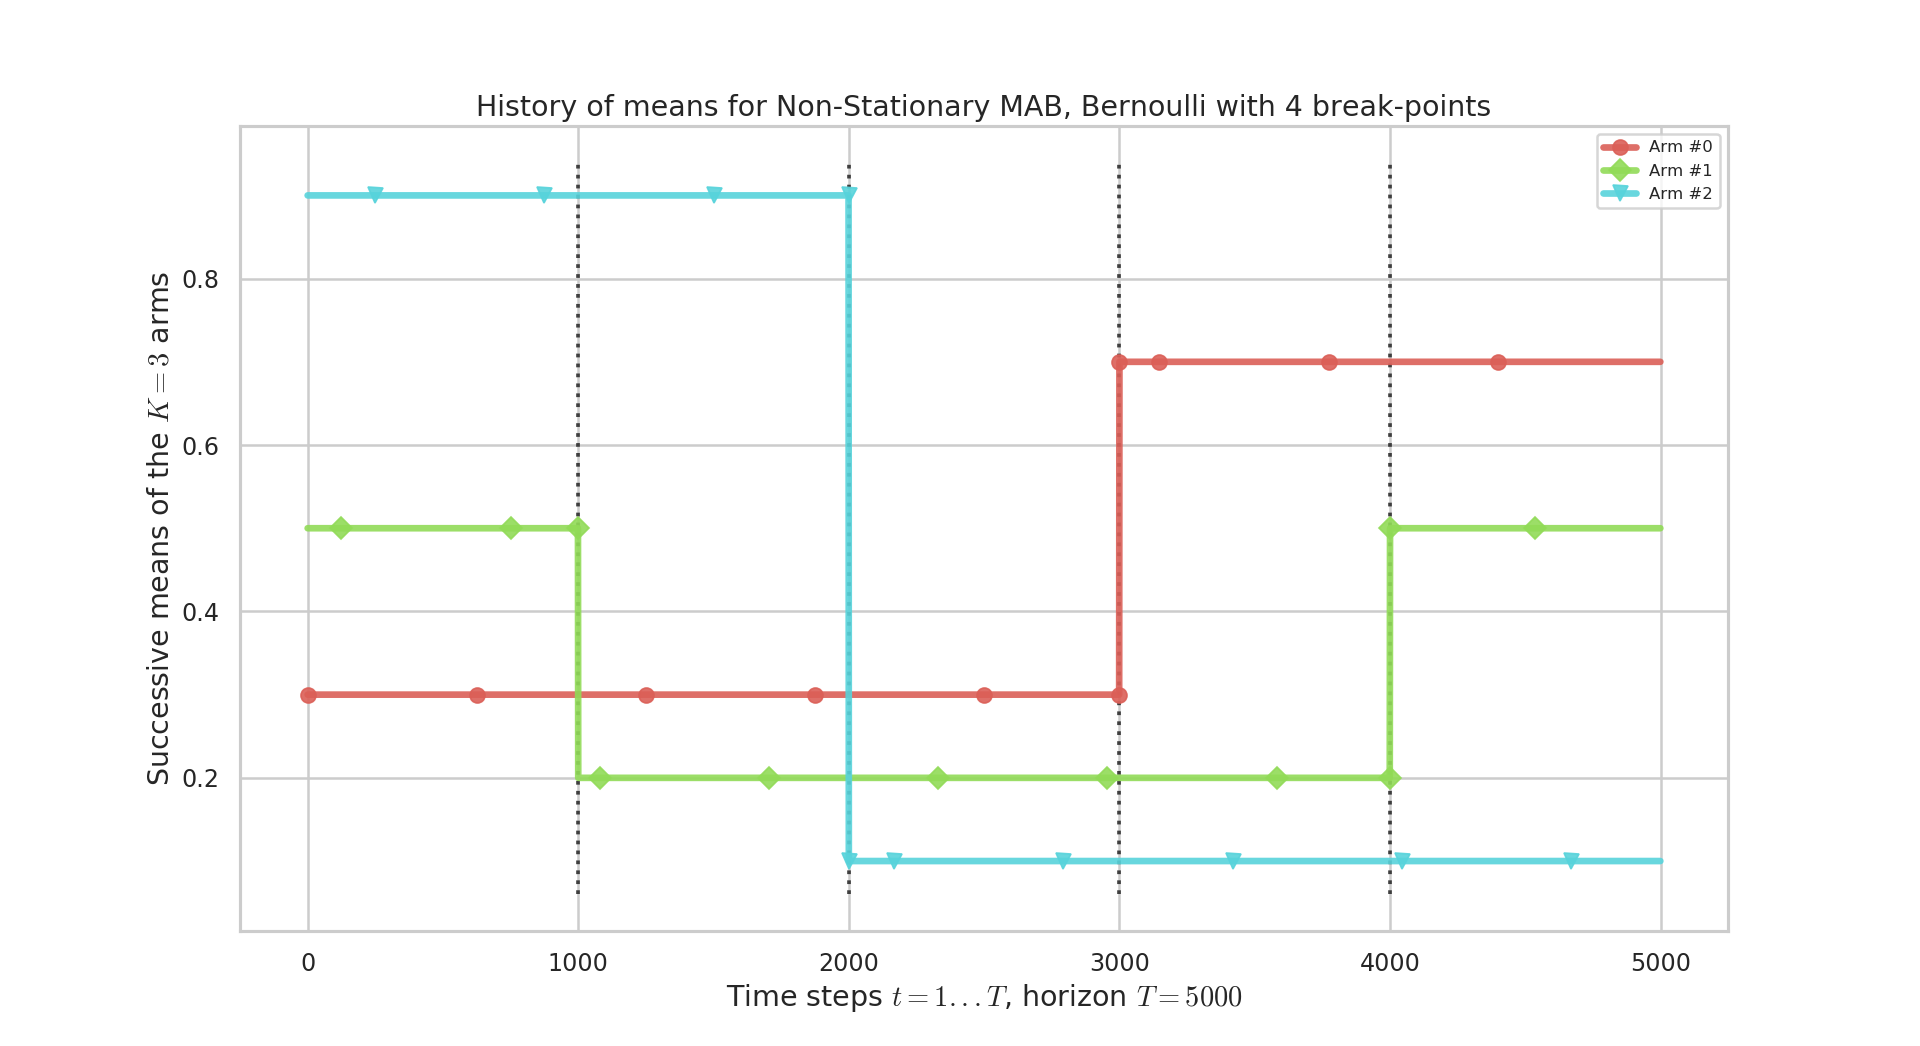
\includegraphics[width=0.80\linewidth]{2-Chapters/6-Chapter/nonstatbandits.git/figures/6_Problems/Problem_1.pdf}
    \subcaption{\textbf{Problem $1$}: $K=3$ arms with $T=5000$, and $\Upsilon=4$ changes occur on only one arm at a time (\ie, $C=4$).}
    \label{fig:6:Problem_1}
\end{figure}

\begin{figure}[h!]  % [htbp]
    \centering
    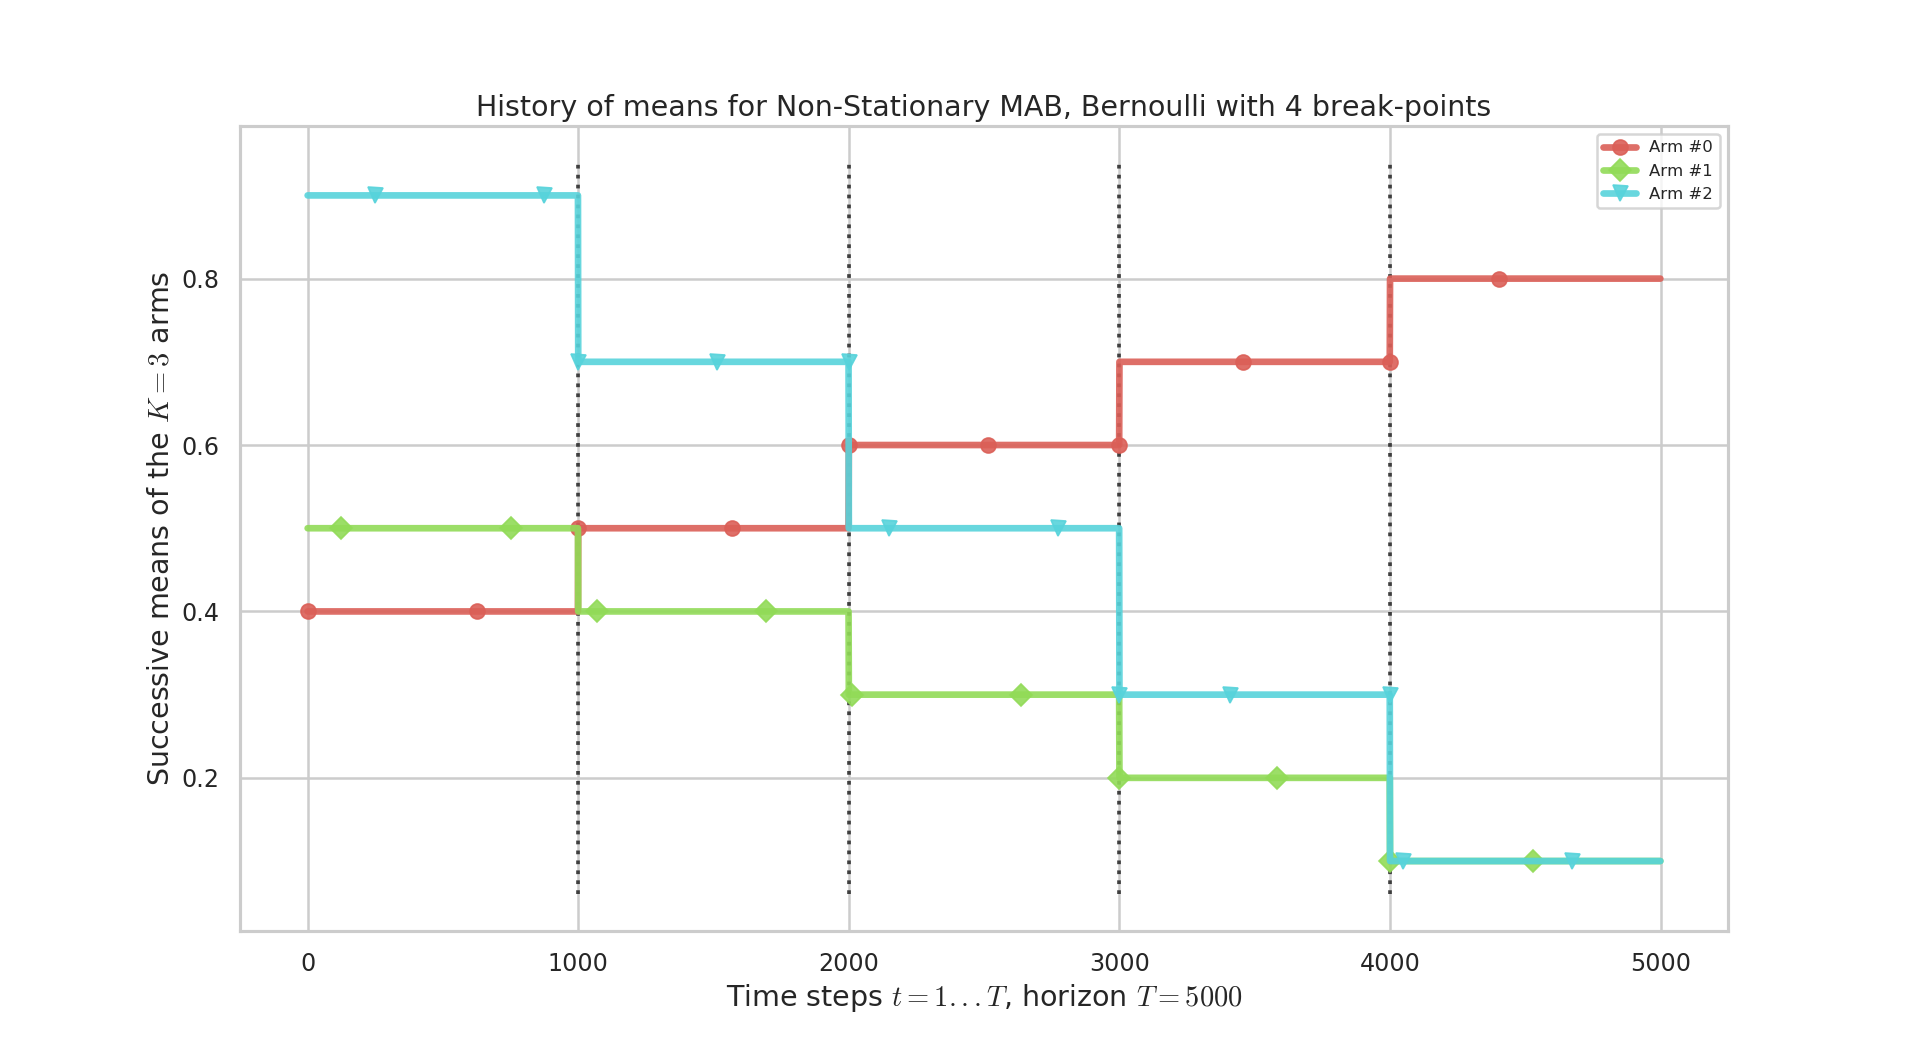
\includegraphics[width=0.80\linewidth]{2-Chapters/6-Chapter/nonstatbandits.git/figures/6_Problems/Problem_2.pdf}
    \subcaption{\textbf{Problem $2$}: $K=3$ arms with $T=5000$, and $\Upsilon=4$ changes occur on all arms (\ie, $C=12$).}
    \label{fig:6:Problem_2}
\end{figure}

\begin{figure}[h!]  % [htbp]
    \centering
    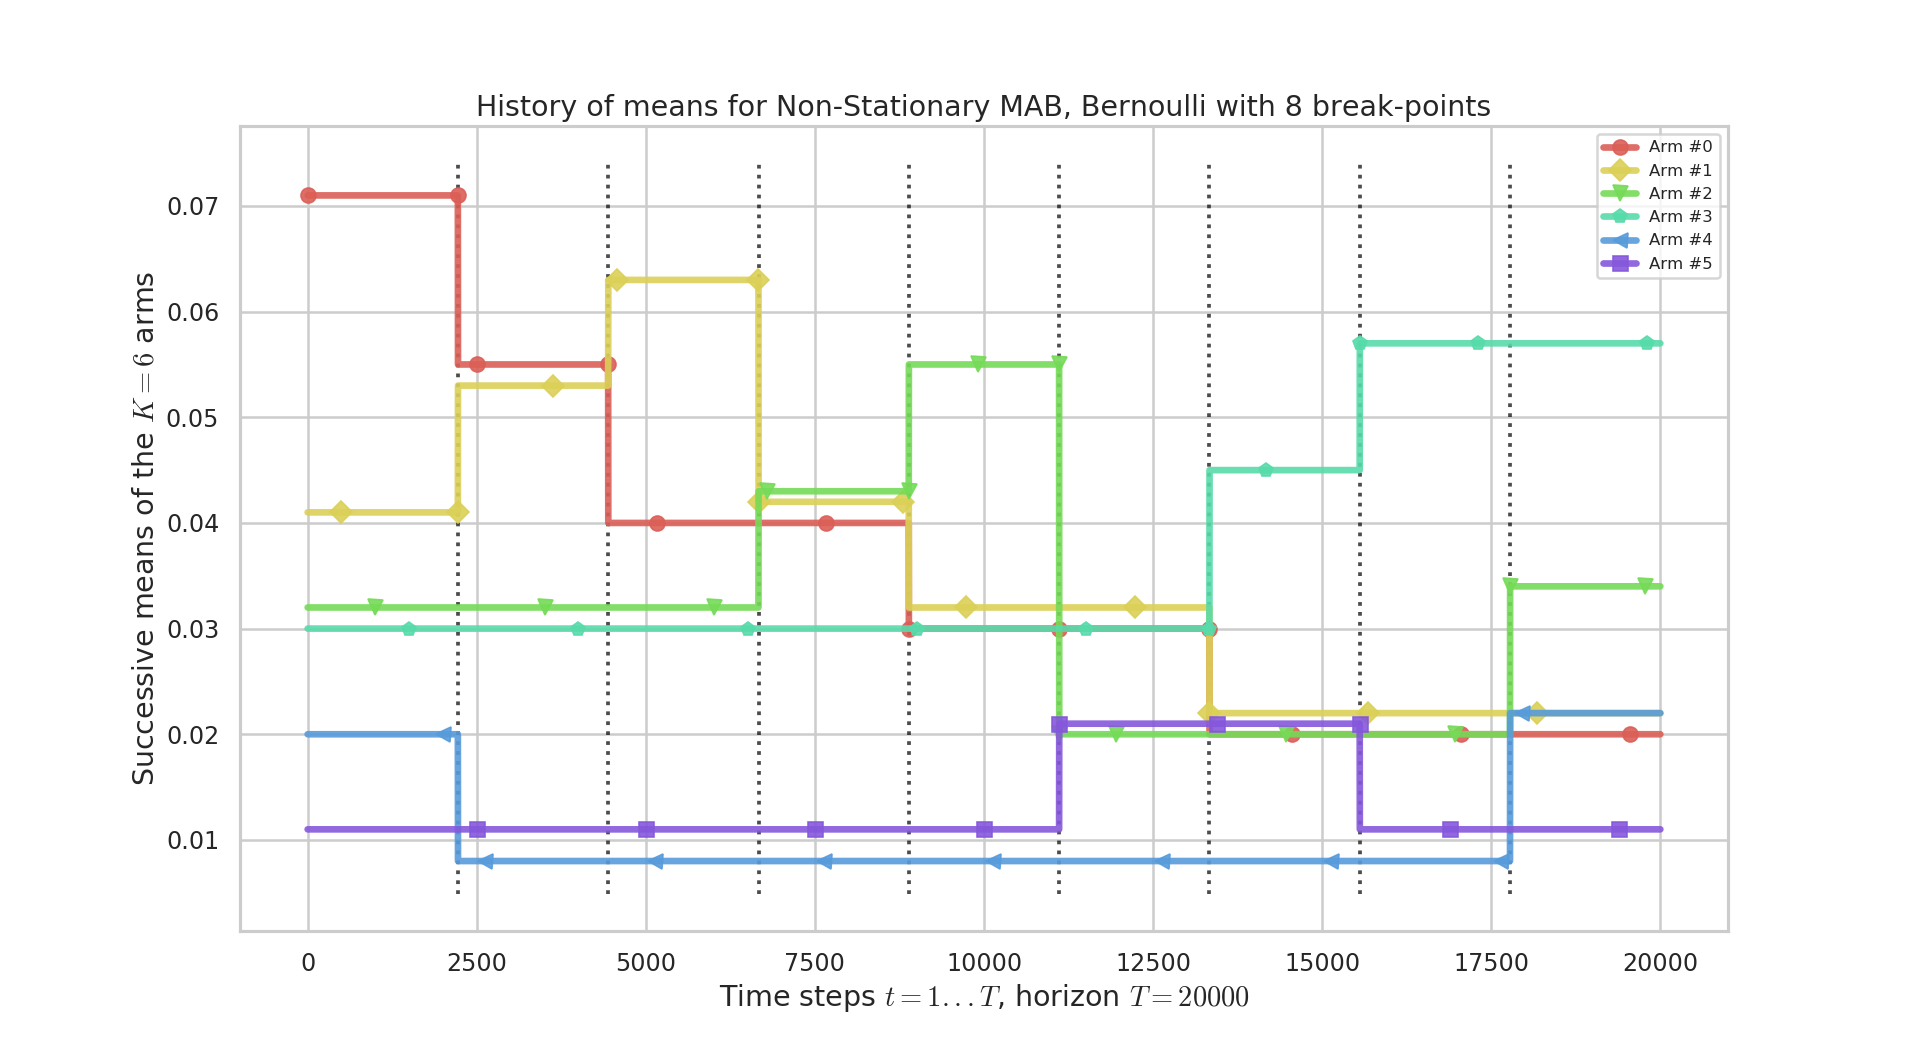
\includegraphics[width=0.80\linewidth]{2-Chapters/6-Chapter/nonstatbandits.git/figures/6_Problems/Problem_5.pdf}
    \subcaption{\textbf{Problem $3$}: $K=6$ arms with $T=20000$, $\Upsilon=8$ changes occur on most arms at a time ($C=19$).
        % Inspired from the Yahoo! example from \cite{CaoZhenKvetonXie18}.
    }
    \label{fig:6:Problem_5}
\end{figure}

%     \caption{History of means of arms for three problems, $\mu_i(t)$ for $i\in\{1,\dots,K\}$ and $t\in\{1,\dots,T\}$.}
%     \label{fig:6:Problems_123}
% \end{figure}


\subsection{Proof of Proposition~\ref{prop:6:EnoughSamples}}\label{proof:6:EnoughSamples}

We consider one arm $i\in\{1,\dots,K\}$, and when the \GLRklUCB{} algorithm is running,
we consider two time steps $s\leq t\in\N^*$, chosen between two restart times for that arm $i$.
Lines~$3$-$4$ state that $A_u = u \mod \lceil \frac{K}{\alpha} \rceil$
if $u \mod \lceil \frac{K}{\alpha} \rceil \in \{1,\dots,K\}$
(see Algorithm~\ref{algo:6:GLRklUCB} for details).
Thus we have
\begin{align*}
    n_i(t) - n_i(s)
    & = \sum_{u=s+1}^{t} \indic(A_u = i) \\
    & \geq \sum_{u=s+1}^{t} \indic\left(A_u = i, A_u = u \mod \left\lceil \frac{K}{\alpha} \right\rceil\right) \\
    & \geq \sum_{u=s+1}^{t} \indic\left(u \mod \left\lceil \frac{K}{\alpha} \right\rceil = i\right) \\
    & = \bigl(t - (s+1) + 1\bigr) / \left\lceil \frac{K}{\alpha} \right\rceil
    \geq \left\lfloor \frac{\alpha}{K} (t - s) \right\rfloor.
\end{align*}
Hence we have the result of Proposition~\ref{prop:6:EnoughSamples}.


% ----------------------------------------------------------------------------
\subsection{Concentration Inequalities}\label{proof:6:Conc}

% ----------------------------------------------------------------------------
\subsubsection{Proof of Lemma~\ref{lem:6:FalseAlarm}} \label{proof:6:FalseAlarm}

Lemma~\ref{lem:6:FalseAlarm} is presented for bounded distributions and is actually valid for any sub-Bernoulli distribution. It could also be presented for more general distributions satisfying
\begin{equation}
    \bE[e^{\lambda X} ] \leq e^{\phi_\mu(\lambda)} \ \ \text{ with } \ \ \mu=\bE[X]\label{def:6:subExpo},
\end{equation}
where $\phi\mu(\lambda)$ is the log moment generating of some one-dimensional exponential family. The Bernoulli divergence $\kl(x,y)$ would be replaced by the corresponding divergence in that exponential family (which is the Kullback-Leibler divergence between two distributions of means $x$ and $y$).

    Let's go back to the Bernoulli case with divergence given in \eqref{eq:6:BernoulliDivergence}. A first key observation is
    \[s \times \kl\left(\hat{\mu}_{1:s},\hat{\mu}_{1:n}\right) + (n-s) \times \kl\left(\hat{\mu}_{s+1:n},\hat{\mu}_{1:n}\right) = \inf_{\mu \in [0,1]}\left[s \times \kl\left(\hat{\mu}_{1:s},\lambda\right) + (n-s) \times \kl\left(\hat{\mu}_{s+1:n},\lambda\right)\right].\]
    Hence the probability of a false alarm occurring is upper bounded as
    %
    \begin{align*}
        \bP_{\mu_0}\left(T_{\delta} < \infty\right) & \leq \bP_{\mu_0}\left(\exists (s,n) \in \N^2, s < n:  s \, \kl\left(\hat{\mu}_{1:s},\hat{\mu}_{1:n}\right) + (n-s) \, \kl\left(\hat{\mu}_{s+1:n},\hat{\mu}_{1:n}\right) > \beta(n,\delta)\right)\\
        & \leq \bP_{\mu_0}\left(\exists (s,n) \in \N^2, s < n:  s \, \kl\left(\hat{\mu}_{1:s},\mu_0\right) + (n-s) \, \kl\left(\hat{\mu}_{s+1:n},\mu_0\right) > \beta(n,\delta)\right) \\
        & \leq \sum_{s =1}^{\infty} \bP_{\mu_0}\left(\exists n > s:  s \, \kl\left(\hat{\mu}_{1:s},\mu_0\right) + (n-s) \, \kl\left(\hat{\mu}_{s+1:n},\mu_0\right) > \beta(n,\delta)\right)\\
        & =   \sum_{s =1}^{\infty} \bP_{\mu_0}\left(\exists r \in \N:  s \, \kl\left(\hat{\mu}_{s},\mu_0\right) + r \, \kl\left(\hat{\mu}'_{r},\mu_0\right) > \beta(s+r,\delta)\right),
    \end{align*}
    where $\hat{\mu}_{s}$ and $\hat{\mu}'_{r}$ are the empirical means of respectively $s$ and $r$ \iid{} observations with mean $\mu_0$ and distribution $\nu$, that are independent from the previous ones.
    As $\nu$ is sub-Bernoulli, the conclusion follows from Lemma~\ref{lem:6:ConcFirst} below and from the definition of $\beta(n,\delta)$:

    \begin{align*}
        &\bP_{\mu_0}\left(T_{\delta} < \infty\right) \\
        & \leq \sum_{s =1}^{\infty} \bP_{\mu_0}\left(\exists r \in \N^* : s \, \kl\left(\hat{\mu}_{s},\mu_0\right) + r \, \kl\left(\hat{\mu}'_{r},\mu_0\right) > 6\ln(1+\ln(s+r))+ 2 \cT\left(\frac{\ln(3(s+r)^{3/2}/\delta)}{2}\right)\right)\\
        & \leq \sum_{s =1}^{\infty} \bP_{\mu_0}\left(\exists r \in \N^* : s \, \kl\left(\hat{\mu}_{s},\mu_0\right) + r \, \kl\left(\hat{\mu}'_{r},\mu_0\right) > 3\ln(1+\ln(s))+3\ln(1+\ln(r)) + 2 \cT\left(\frac{\ln(3s^{3/2}/\delta)}{2}\right)\right)
    \end{align*}
    And so we have $\bP_{\mu_0}\left(T_{\delta} < \infty\right) \leq \sum_{s =1}^{\infty} \frac{\delta}{3s^{3/2}} \leq \delta$.

    \begin{lemma}\label{lem:6:ConcFirst}
    $(X_i)_{i \in \N}$ and $(Y_i)_{i \in \N}$ two independent \iid{} processes with resp. means $\mu$ and $\mu'$ such that
    \[\bE[e^{\lambda X_1}] \leq e^{\phi_{\mu}(\lambda)} \ \ \text{and} \ \ \bE[e^{\lambda Y_1}] \leq e^{\phi_{\mu'}(\lambda)},\]
    where $\phi_\mu(\lambda) = \bE_{X \sim \nu^{\mu}}[e^{\lambda X}]$ is the moment generating function of the distribution $\nu^\mu$, which is the unique distribution in an exponential family that has mean $\mu$.
    %
    Let $\kl(\mu,\mu') = \KL(\nu^\mu,\nu^{\mu'})$ be the divergence function associated to that exponential family. Introducing the notation $\hat{\mu}_s = \frac{1}{s}\sum_{i=1}^s X_i$ and $\hat{\mu}'_r = \frac{1}{r}\sum_{i=1}^r Y_i$, it holds that for every $s,r \in \N^*$,
    \[\bP\left(\exists r \in \N^* : s \, \kl\left(\hat{\mu}_{s},\mu\right) + r \, \kl\left(\hat{\mu}_r',\mu'\right) > 3\ln(1+\ln(s)) + 3\ln(1+\ln(r)) + 2\cT\left(\frac{x}{2}\right)\right)\leq e^{-x},\]
    where $\cT$ is the function defined in \eqref{def:6:function_T}.
\end{lemma}

\paragraph{Proof of Lemma~\ref{lem:6:ConcFirst}.}
Using the same construction as in the proof of Theorem~14 in \cite{KK18Martingales}, one can prove that for every $\lambda \in I$ (for an interval $I$), there exists a non-negative super-martingale $M^\lambda (s)$ with respect to the filtration $\cF_t = \sigma(X_1,\dots,X_t)$ that satisfies $\bE[M^\lambda(s)] \leq 1$ and
\[\forall s \in \N^*, \ \ M^\lambda (s) \geq e^{\lambda [s\kl(\hat{\mu}_s,\mu) - 3\ln(1+\ln(s))] - g(\lambda)}\]
for some function $g : I \rightarrow \R$. This super-martingale is of the form
\[M^\lambda (s) = \int e^{\eta\sum_{i=1}^s X_i - \phi_\mu(\lambda)s} d\pi(\eta)\]
for a well-chosen probability distribution $\pi$, and the function $g$ can be chosen to be any
\begin{small}
\begin{eqnarray*}
    g_{\xi} : \left[0; 1/(1+\xi)\right] & \longrightarrow & \R \\
    \lambda & \mapsto & \lambda(1+\xi) \ln \left(\frac{\pi^2}{3(\ln(1+\xi))^2}\right) -  \ln(1 - \lambda(1 + \xi))
\end{eqnarray*}
\end{small}
for a parameter $\xi \in [0,1/2]$.

Similarly, there exists an independent super-martingale $W^\lambda (r)$ w.r.t. the filtration $\cF_r' = \sigma(Y_1,\dots,Y_r)$ such that
\[\forall r \in \N^*, \ \ W^\lambda (r) \geq e^{\lambda [r\kl(\hat{\mu}'_r,\mu) - 3\ln(1+\ln(r))] - g(\lambda)},\]
for the same function $g(\lambda)$. In the terminology of \cite{KK18Martingales}, the processes $\bm{X}(s) = s \, \kl(\hat{\mu}_s,\mu) - 3\ln(1+\ln(s))$ and $\bm{Y}(s) = r \, \kl(\hat{\mu}_r,\mu) - 3\ln(1+\ln(r))$ are called $g$-DCC for Doob-Cram\'er-Chernoff, as Doob's inequality can be applied in combination with the Cram\'er-Chernoff method to obtain deviation inequalities that are uniform in time.

Here we have to modify the technique used in their Lemma 4 in order to take into account the two stochastic processes, and the presence of super-martingales instead of martingales (for which Doob inequality still works). One can write
\begin{align*}
    &\bP\left(\exists r \in \N^* : s \, \kl\left(\hat{\mu}_{s},\mu\right) + r \, \kl\left(\hat{\mu}_r',\mu'\right) > 3\ln(1+\ln(s)) + 3\ln(1+\ln(r)) + u\right) \\
    & \leq \bP\left(\exists r \in \N^* : M^\lambda(s)W^\lambda(r) > e^{\lambda u - 2g(\lambda)}\right) \\
    & = \lim_{n \rightarrow \infty} \bP\left(\exists r \in \{1,\dots,n\} :  M^\lambda(s)W^\lambda(r) > e^{\lambda u - 2g(\lambda)}\right) \\
    & = \lim_{n \rightarrow \infty} \bP\left(\sup_{r \in \{1,\dots,n\}}  M^\lambda(s)W^\lambda(r) > e^{\lambda u - 2g(\lambda)}\right).
\end{align*}
%
Using that $\tilde{M}(r) = M^\lambda(s)W^\lambda(r)$ is a super-martingale with respect to the filtration \[\tilde{\cF}_r = \sigma(X_1,\dots,X_s, Y_1,\dots,Y_r),\] one can apply Doob's maximal inequality to obtain
\begin{eqnarray*}
    \bP\left(\sup_{r \in \{1,\dots,n\}}  M^\lambda(s)W^\lambda(r) > e^{\lambda u - 2g(\lambda)}\right) &\leq& e^{-(\lambda u - 2g(\lambda))}\bE[\tilde{M}(1))] \\
    & = & e^{-(\lambda u - 2g(\lambda))}\bE[M^\lambda(s)W^\lambda(1)] \\
    & \leq & e^{-(\lambda u - 2g(\lambda))},
\end{eqnarray*}
using that $M^\lambda(s)$ and $W^\lambda(1)$ are independent and have an expectation smaller than $1$.

Putting things together yields
\[\bP\left(\exists r \in \N^* : s \, \kl\left(\hat{\mu}_{s},\mu\right) + r \, \kl\left(\hat{\mu}_r',\mu'\right) > 3\ln(1+\ln(s)) + 3\ln(1+\ln(r)) + u\right) \leq e^{-\left(\lambda u - 2g_{\xi}(\lambda)\right)},\]
for any function $g_{\xi}$ defined above.
%
The conclusion follows by optimizing for both $\lambda$ and $\xi$, using Lemma~18 in \cite{KK18Martingales}.


% ----------------------------------------------------------------------------
\subsubsection{A Concentration Result Involving Two Arms}\label{proof:6:Chernoff2arms}

The following result is useful to control the probability of the good event in our two regret analyzes. Its proof follows from a straightforward application of the Cram\'er-Chernoff method (\cite{Boucheron2013}).

\begin{lemma}\label{lem:6:Chernoff2arms}
    Let $\hat{\mu}_{i,s}$ be the empirical mean of $s$ \iid{} observations with mean $\mu_i$, for $i \in \{a,b\}$, that are $\sigma^2$-sub-Gaussian. Define $\Delta = \mu_a - \mu_b$. Then for any $s,r > 0$, we have
    \begin{eqnarray*}
        \bP\left(\frac{sr}{s+r}\Big(\hat{\mu}_{a,s} - \hat{\mu}_{b,r} - \Delta\Big)^2 \geq u \right) &\leq& 2\exp\left(- \frac{u}{2\sigma^2}\right)\cdot
    \end{eqnarray*}
\end{lemma}

\paragraph{Proof of Lemma~\ref{lem:6:Chernoff2arms}.}

We first note that
\begin{align}\label{eq:6:Preparation}
	&\bP\left(\frac{sr}{s+r}\Big(\hat{\mu}_{a,s} - \hat{\mu}_{b,r} - \Delta\Big)^2 \geq u \right) \nonumber\\
	&\leq \bP\left(\hat{\mu}_{a,s} - \hat{\mu}_{b,r} \geq \Delta + \sqrt{\frac{s+r}{sr}u} \right) + \bP\left(\hat{\mu}_{b,r} - \hat{\mu}_{a,s} \geq -\Delta + \sqrt{\frac{s+r}{sr}u} \right),
\end{align}
and those two quantities can be upper-bounded similarly using the Cram\'er-Chernoff method.

Let $(X_i)$ and $(Y_i)$ be two \iid{} sequences that are $\sigma^2$ sub-Gaussian with mean $\mu_1$ and $\mu_2$ respectively. Let $n_1$ and $n_2$ be two integers and $\hat\mu_{1,n_1}$ and $\hat{\mu}_{2,n_2}$ denote the two empirical means based on $n_1$ observations from $X_i$, and $n_2$ observations from $Y_i$ respectively.
Then for every $\lambda > 0$, we have
\begin{eqnarray*}
    \bP\left(\hat\mu_{1,n_1} - \hat\mu_{2,n_2} \geq \mu_1 - \mu_2 + x \right) & \leq & \bP\left(\frac{1}{n_1}\sum_{i=1}^{n_1} (X_i-\mu_1) - \frac{1}{n_2}\sum_{i=1}^{n_2} (Y_i - \mu_2) \geq x \right)\\
    & \leq & \bP\left(e^{\lambda \left(\frac{1}{n_1}\sum\limits_{i=1}^{n_1} (X_i-\mu_1) - \frac{1}{n_2}\sum\limits_{i=1}^{n_2} (Y_i - \mu_2)\right)} \geq e^{\lambda x} \right) \\
    \text{(using Markov's inequality)}
    & \leq & e^{-\lambda x}\bE\left[e^{\lambda \frac{1}{n_1}\sum\limits_{i=1}^{n_1} (X_i-\mu_1)}\right]\bE\left[e^{-\lambda \frac{1}{n_2}\sum\limits_{i=1}^{n_2} (Y_i-\mu_2)}\right] \\
    & = & \exp\left(- \lambda x + n_1\phi_{X_1 - \mu_1}\left(\frac{\lambda}{n_1}\right) + n_2\phi_{Y_1 - \mu_2}\left(-\frac{\lambda}{n_2}\right)\right) \\
    & \leq & \exp\left(- \lambda x + \frac{\lambda^2\sigma^2}{2n_2} + \frac{\lambda^2\sigma^2}{2n_1}\right),
\end{eqnarray*}
%
where the last inequality uses the sub-Gaussian property.
%
Choosing the value $\lambda = \frac{x}{2\left[\sigma^2/(2n_1) + \sigma^2/(2n_2)\right]}$ which minimizes the right-hand side of the inequality yields
\[\bP\left(\hat\mu_{1,n_1} - \hat\mu_{2,n_2} \geq \mu_1 - \mu_2 + x \right) \leq \exp\left(- \frac{n_1n_2}{n_1+n_2}\frac{x^2}{2\sigma^2}\right).\]
Using this inequality twice in the right hand side of \eqref{eq:6:Preparation} concludes the proof.


% ----------------------------------------------------------------------------
\subsection{Analysis of \GLRklUCB{} with Global Changes}\label{proof:6:mainRegretBoundGlobal}

We gave in Section~\ref{sec:6:RegretAnalysis} the following decomposition of the regret $R_T$,
\begin{eqnarray}\label{eq:6:GeneRegretBound}
    R_T &\leq& T \bP\left(\cE_T^c\right) + \alpha T + \underbrace{\bE\left[\indic(\cE_T) \sum_{t=1}^T \indic\left(\UCB_{i^*_t}(t) \leq \mu_{i^*_t}(t)\right)\right]}_{(A)} \nonumber \\
    & & + \underbrace{\bE\left[\indic(\cE_T)\sum_{t=1}^T (\mu_{i^*_t}(t) - \mu_{I_t}(t))\indic\left(\UCB_{I_t}(t) \geq \mu_{i^*_t}(t)\right)\right]}_{(B)}.
\end{eqnarray}


\subsubsection{Proof of Theorem~\ref{thm:6:mainRegretBoundGlobal}.}

We first introduce some notation for the proof:
let $\hat\tau^{(k)}$ be the $k$-th change detected by the algorithm, leading to the $k$-th (full) restart and let $\hat\tau(t)$ be the last time before $t$ that the algorithm restarted.
We denote $n_i(t) = \sum_{s=\tau(t)+1}^{t}\indic(A_s = i)$ the number of selections of arm $i$ since the last (global) restart, and $\hat{\mu}_i(t) = \frac{1}{n_i(t)}\sum_{s=\tau(t)+1}^{t}X_{i,s}\indic(A_s = i)$ their empirical average (if $n_i(t) \neq 0$).

As explained before, our analysis relies on the general regret decomposition~\eqref{eq:6:GeneRegretBound}, with the following appropriate good event. Let $d^k$ be defined as in Assumption~\ref{ass:6:LongPeriodsGlobal}, we define
\begin{equation}\cE_T(\delta) = \left( \forall k \in \{1, \ldots, \Upsilon_T\}, \hat{\tau}^{(k)} \in \left[\tau^{(k)} + 1, \tau^{(k)} + d^{(k)}\right] \right).\label{def:6:GoodEvenGlobal}\end{equation}
Under the good event, all the change points are detected within a delay at most $d^(k)$.
%
Note that from Assumption~\ref{ass:6:LongPeriodsGlobal}, as the period between two changes are long enough, if $\cE_T(\delta)$ holds, then for all change $k$, one has $\tau^{(k)} \leq \hat{\tau}^{(k)} \leq \tau^{(k+1)}$. Using Assumption~\ref{ass:6:LongPeriods}, one can prove the following.

\begin{lemma}\label{lem:6:GoodEventGlobal}
    With $\cE_T(\delta)$ defined as in \eqref{def:6:GoodEvenGlobal}, the ``bad event'' is unlikely:
    $\bP(\cE_T^c(\delta)) \leq \delta(K+1)\Upsilon_T$.
\end{lemma}

We now turn our attention to upper bounding the two terms $(A)$ and $(B)$ in \eqref{eq:6:GeneRegretBound}.


\paragraph{Upper bound on Term $\bm{(A)}$}

\begin{align*}
    (A) & \leq \bE\left[\indic(\cE_T) \sum_{t=1}^T \indic\left(n_{i_t^*}(t) \, \kl\left(\hat{\mu}_{i_t^*}(t), \mu_{i_t^*}(t)\right) \geq f(t - \tau(t))\right)\right] \\
     & \leq \sum_{k=1}^{\Upsilon_T}\bE\left[\indic(\cE_T) \sum_{t=\tau^{(k)}+1}^{\tau^{(k+1)}} \indic\left(n_{k^*}(t) \, \kl\left(\hat{\mu}_{k^*}(t), \mu_{k^*}^{(k)}\right) \geq f(t - \hat\tau(t))\right)\right] \\
    & \leq \sum_{k=1}^{\Upsilon_T}\bE\left[ d^{(k)} + \indic(\cE_T) \sum_{t=\hat{\tau}^{(k)}+1}^{\tau^{(k+1)}} \indic\left(n_{k^*}(t) \, \kl\left(\hat{\mu}_{k^*}(t), \mu_{k^*}^{(k)}\right) \geq f(t - \hat\tau^{(k)})\right)\right] \\
    & \leq \sum_{k=1}^{\Upsilon_T}d^{(k)} + \sum_{k=1}^{\Upsilon_T}\bE\left[\indic(\cC^{(k)}) \sum_{t=\hat{\tau}^{(k)}}^{\tau^{(k+1)}}\indic\left(n_{k^*}(t) \, \kl\left(\hat{\mu}_{k^*}(t), \mu_{k^*}\right) \geq f(t - \hat\tau^{(k)})\right)\right],
\end{align*}
%
where we introduce the event $\cC^{(k)}$ that all the changes up to the $k$-th have been detected:
%
\begin{equation}\label{def:6:EventCiGlobal}
    \cC^{(k)} = \left\{\forall j \leq k, \hat\tau^{(j)} \in \{\tau^{(j)} + 1, \dots, \tau^{(j)} + d^{(j)} \} \right\}.
\end{equation}
%
Clearly, $\cE_T \subseteq \cC^{(k)}$ and $\cC^{(k)}$ is $\cF_{\hat\tau^{(k)}}$-measurable. Observe that conditionally to $\cF_{\hat\tau^{(k)}}$, when $\cC^{(k)}$ holds, $\hat{\mu}_{k^*}(t)$ is the average of samples that have all mean $\mu_{k^*}^{(k)}$.
%
Thus, introducing $\hat{\mu}_s$ as a sequence of \iid{} random variables with mean $\mu_{k^*}^{(k)}$, one can write
%
\begin{align*}
    &\bE\left[\left.\indic(\cC^{(k)}) \sum_{t=\hat{\tau}^{(k)}}^{\tau^{(k+1)}} \indic\left(n_{k^*}(t) \, \kl\left(\hat{\mu}_{k^*}(t), \mu_{k^*}^{(k)}\right) \geq f(t - \hat\tau^{(k)})\right) \right| \cF_{\hat\tau^{(k)}}\right]\\
    & = \indic(\cC^{(k)}) \sum_{t=\hat{\tau}^{(k)}}^{\tau^{(k+1)}} \bE\left[\indic\left(n_{k^*}(t) \, \kl\left(\hat{\mu}_{k^*}(t), \mu_{k^*}^{(k)}\right) \geq f(t - \hat\tau^{(k)})\right) \;|\; \cF_{\hat\tau^{(k)}}\right] \\
    & \leq \indic(\cC^{(k)}) \sum_{t'=1}^{\tau^{(k+1)} - \hat{\tau}^{(k)}} \bP\left(\exists s \leq t' : s \, \kl(\hat{\mu}_{s},\mu_{k^*}^{(k)}) \geq f(t')\right) \\
    & \leq \sum_{t=1}^T \frac{1}{t\ln(t)} \leq \ln(\ln(T)),
\end{align*}
%
where the last but one inequality relies on the concentration inequality given in Lemma 2 of \cite{KLUCBJournal} and the fact that $f(t) = \ln(t) + 3 \ln(\ln(t))$. Finally, using the law of total expectation yields
\begin{equation}\label{eq:6:TermAFinalGlobal}
    (A) \leq \sum_{k=1}^{\Upsilon_T}\left[d^{(k)} + \ln(\ln(T))\right].
\end{equation}

\paragraph{Upper bound on Term $\bm{(B)}$.} We let $\tilde{\mu}_{i,s}^{(k)}$ denote the empirical mean of the first $s$ observations of arm $i$ made after time $t=\hat{\tau}^{(k)}+1$. Rewriting the sum in $t$ as the sum of consecutive intervals $[\tau^{(k)}+1, \tau^{(k+1)}]$,
\begin{align*}
    (B) & \leq \bE\Big[\indic(\cE_T)\sum_{k=1}^{\Upsilon_T} \sum_{t=\tau^{(k)}}^{\tau^{(k+1)}}\left(\mu_{k^*}^{(k)} - \mu_{I_t}^{(k)}\right)\indic\left(\UCB_{I_t}(t) \geq \mu_{k^*}^{(k)}\right)\Big] \\
     & \leq \sum_{k=1}^{\Upsilon_T}\bE\Big[\indic(\cE_T)\hat{\tau}^{(k)} + \indic(\cE_T) \sum_{t=\hat\tau^{(k)}+1}^{\tau^{(k+1)}}\left(\mu_{k^*}^{(k)} - \mu_{I_t}^{(k)}\right)\indic\left(\UCB_{I_t}(t) \geq \mu_{k^*}^{(k)}\right)\Big] \\
    & \leq \sum_{k=1}^{\Upsilon_T}d_i^{(k)}+ \sum_{i=1}^K \bE\Big[\indic(\cE_T) \sum_{t=\hat\tau^{(k)}+1}^{\tau^{(k+1)}}\left(\mu_{k^*}^{(k)} - \mu_{i}^{(k)}\right)\indic\left(I_t=i,\UCB_{i}(t) \geq \mu_{k^*}^{(k)}\right)\Big] \\
     & \leq \sum_{k=1}^{\Upsilon_T}d_i^{(k)}+ \sum_{i=1}^K \sum_{k=1}^{\Upsilon_T}\left(\mu_{k^*}^{(k)} - \mu_{i}^{(k)}\right)\times \\
     &\hspace{1cm}\bE\Big[\indic(\cE_T) \sum_{t=\hat{\tau}^{(k)}+1}^{\tau^{(k+1)}}\sum_{s=1}^{t-\hat\tau^{(k)}}\indic\left(I_t = i,n_i(t) = s\right) \indic\left(s \, \kl(\tilde{\mu}_{i,s}^{(k)}, \mu_{k^*}^{(k)}) \leq f(\tau^{(k+1)} - \hat\tau^{(k)})\right)\Big] \\
    & \leq \sum_{k=1}^{\Upsilon_T}d_i^{(k)}+ \sum_{i=1}^K \sum_{k=1}^{\Upsilon_T}\left(\mu_{k^*}^{(k)} - \mu_{i}^{(k)}\right)\bE\Big[\indic(\cE_T) \sum_{s=1}^{n_i(\tau^{(k+1)})}\indic\left(s \, \kl(\tilde{\mu}_{i,s}^{(k)}, \mu_{k^*}^{(k)}) \leq f(\tau^{(k+1)} - \tau^{(k)})\right)\Big]  \\
    & \leq \sum_{k=1}^{\Upsilon_T}d_i^{(k)}+ \sum_{i=1}^K \sum_{k=1}^{\Upsilon_T}\left(\mu_{k^*}^{(k)} - \mu_{i}^{(k)}\right)\bE\Big[\indic(\cC^{(k)}) \sum_{s=1}^{n_i(\tau^{(k+1)})}\indic\left(s \, \kl(\tilde{\mu}_{i,s}^{(k)}, \mu_{k^*}^{(k)}) \leq f(\tau^{(k+1)} - \tau^{(k)})\right)\Big].
\end{align*}

Conditionally to $\cF_{\hat\tau^{(k)}}$, when $\cC^{(k)}$ holds, for $s \in \{1, \ldots, n_i(\tau^{(k+1)})\}$, $\tilde{\mu}_{i,s}^{(k)}$ is the empirical mean from \iid{} observations of mean $\mu_i^{(k)}$.
Therefore, introducing $\hat{\mu}_s$ as a sequence of \iid{} random variables with mean $\mu_i^{(k)}$, it follows from the law of total expectation that
\begin{align*}
    (B)& \leq \sum_{k=1}^{\Upsilon_T}d^{(k)}+\sum_{i=1}^K\sum_{k=1}^{\Upsilon_T}\left(\mu_{k^*}^{(k)} - \mu_{i}^{(k)}\right) \sum_{s=1}^{\tau^{(k+1)}-\tau^{(k)}}\bP\left(s \times \kl(\hat{\mu}_{s}, \mu_{k^*}^{(k)}) \leq f(\tau^{(k+1)} - \tau^{(k)})\right)\cdot
\end{align*}
If $\mu_{k^*}^{(k)} > \mu_i^{(k)}$ by definition, we can use the analysis of \klUCB{} from \cite{KLUCBJournal} to further upper bound the right-most part, and we obtain
\begin{align}\label{eq:6:TermBFinalGlobal}
    (B) & \leq \sum_{k=1}^{\Upsilon_T}d^{(k)}+\sum_{i=1}^K\sum_{k=1}^{\Upsilon_T}\indic\left(\mu_i^{(k)} \neq \mu_{k^*}^{(k)}\right)\left[ \frac{\left(\mu_{k^*}^{(k)} - \mu_{i}^{(k)}\right)}{\kl(\mu_i^{(k)},\mu_{k^*}^{(k)})}\log(T) + \bigO{\sqrt{\log(T)}}\right].
\end{align}

Combining the regret decomposition~\eqref{eq:6:GeneRegretBound} with Lemma~\ref{lem:6:GoodEventGlobal} and the two upper bounds in \eqref{eq:6:TermAFinalGlobal} and \eqref{eq:6:TermBFinalGlobal},
\[R_T \leq 2\sum_{k=1}^{\Upsilon_T} \frac{4K}{\alpha \left(\Delta^{(k)}\right)^2}\beta(T,\delta) +\alpha T + \delta (K+1)\Upsilon_T  + \sum_{k=1}^{\Upsilon_T}\sum_{i : \mu_i^{(k)} \neq \mu_{k^*}^{(k)}} \frac{\left( \mu_{k^*}^{(k)}-\mu_i^{(k)}\right)}{\kl\left(\mu_i^{(k)},\mu_{k^*}^{(k)}\right)}\ln(T) + \bigO{\sqrt{\ln(T)}},\]
which concludes the proof.

\subsubsection{Controlling the probability of the good event: Proof of Lemma~\ref{lem:6:GoodEventGlobal}}

% We introduce $\hat{\mu}_{i,s}^{(k)}$ as the empirical mean of the first $s$ observations of arm $i$ made after $t=\tau^{(k)}+1$ and $\tilde{\mu}_{i,s}^{(k)}$ as the empirical mean of the first $s$ observations of arm $i$ made after time $t=\hat{\tau}^{(k)}+1$.

Recall that $\cC^{(k)}$ defined in \eqref{def:6:EventCiGlobal} is the event that all the breakpoints up to the $k$-th have been correctly detected.
Using a union bound, one can write
%
\begin{align*}
    \bP(\cE_T^c) & \leq \sum\limits_{k=1}^{\Upsilon_T}
    \bP\left(\left. \hat\tau^{(k)} \notin \{ \tau^{(k)}+1, \dots, \tau^{(k)} + d^{(k)} \} \right|\; \cC^{(k-1)}\right) \\
    \\ & \leq \sum\limits_{k=1}^{\Upsilon_T} \underbrace{\bP\left(\hat\tau^{(k)} \leq \tau^{(k)} \;|\; \cC^{(k-1)}\right)}_{(a)} + \sum\limits_{k=1}^{\Upsilon_T} \underbrace{\bP\left(\hat\tau^{(k)} \geq \tau^{(k)} + d^{(k)} \;|\; \cC^{(k-1)}\right)}_{(b)}.
\end{align*}
%
The final result follows by proving that $(a) \leq K \delta$ and $(b)\leq \delta$, as detailed below.


\paragraph{Upper bound on $(a)$: controlling the false alarm.}
%
$\hat\tau^{(k)} \leq \tau^{(k)}$ implies that there exists an arm whose associated change point detector has experienced a false-alarm:
%
\begin{align*}
    (a) & \leq \bP\left(\exists i, \exists s < t \leq n_i(\tau_i^{(k)}) : s \, \kl\left(\tilde{\mu}_{i,1:s}^{(k-1)},\tilde{\mu}_{i,1:t}^{(k-1)}\right) + (t - s) \, \kl\left(\tilde{\mu}_{i,s+1:t}^{(k-1)},\tilde{\mu}_{i,1:t}^{(k-1)}\right) > \beta(t, \delta) \;|\; \cC^{(k-1)}\right) \\
    & \leq \sum_{i=1}^K\bP\left(\exists s < t : s \, \kl(\hat{\mu}_{1:s},\mu_i^{(k-1)}) + (t - s) \, \kl(\hat{\mu}_{s+1:t}, \mu_{i}^{(k-1)}) > \beta(t, \delta)\right),
\end{align*}
with $\hat\mu_{s:s'} = \sum_{r=s}^{s'} Z_{i,r}$ where $Z_{i,r}$ is an \iid{} sequence with mean $\mu_i^{(k-1)}$.
Indeed, conditionally to $\cC^{(k-1)}$, the $n_i(\tau^{(k)})$ successive observations of arm $i$ arm starting from $\hat \tau^{(k)}$ are \iid{} with mean $\mu_i^{(k-1)}$.
Using Lemma~\ref{lem:6:ConcFirst}, term $(a)$ is upper bounded by $K\delta$.


\paragraph{Upper bound on term (b): controlling the delay.}
%
From the definition of $\Delta^{(k)}$, there exists an arm $i$ such that $\Delta^{(k)} = |\mu_i^{(k)} - \mu_i^{(k-1)}|$. We shall prove that it is unlikely that the change-point detector associated to $i$ doesn't trigger within the delay $d^{(k)}$.

First, it follows from Proposition~\ref{prop:6:EnoughSamples} that there exists $\overline{t} \in \{\tau^{(k)}, \dots, \tau^{(k)} + d^{(k)} \}$ such that
$n_i(\overline{t}) - n_i(\tau^{(k)}) = \overline{r}$ where $\overline{r} = \lfloor \frac{\alpha}{K} d^{(k)}\rfloor$
(as the mapping $t\mapsto n_i(t) - n_i(\tau^{(k)})$ is non-decreasing, is $0$ at $t=\tau^{(k)}$ and its value at $\tau^{(k)}+d^{(k)}$ is larger than $\overline{r}$).  Using that \[\left(\hat\tau^{(k)} \geq \tau^{(k)} + d^{(k)}\right) \subseteq \left(\hat\tau^{(k)} \geq \overline{t}\right)\]
the event $\left(\hat\tau^{(k)} \geq \tau^{(k)} + d^{(k)}\right)$ further implies that
\[
    n_i(\tau^{(k)}) \, \kl\left(\tilde{\mu}^{k-1}_{i,n_i(\tau^{(k)})},\tilde{\mu}^{k-1}_{i,n_i(\overline{t})}\right)
    + \overline{r} \, \kl\left(\tilde{\mu}^{k-1}_{i,n_i(\tau^{(k)}) : n_i(\overline{t})},\tilde{\mu}^{k-1}_{i,n_i(\overline{t})}\right) \leq \beta(n_i(\tau^{(k)}) + \overline{r},\delta),
\]
where $\tilde{\mu}^{k-1}_{i,s}$ denotes the empirical mean of the $s$ first observation of arm $i$ since the $(k-1)$-th restart $\hat{\tau}^{(k-1)}$ and  $\tilde{\mu}^{k-1}_{i,s:s'}$ the empirical mean that includes observation number $s$ to number $s'$. Conditionally to $\cC^{(k-1)}$, $\tilde{\mu}^{k-1}_{i,n_i(\tau^{(k)})}$ is the empirical mean of $n_i(\tau^{(k)})$ \iid{} replications of mean $\mu^{k-1}$, whereas $\tilde{\mu}^{k-1}_{i,n_i(\tau^{(k)}) : n_i(\overline{t})}$ is the empirical mean of $\overline{r}$ \iid{} replications of mean $\mu_i^{k}$.

Moreover, due to Proposition~\ref{prop:6:EnoughSamples}, $n_i(\tau^{(k)})$ lies in the interval $
\left[\left\lfloor \frac{\alpha}{K}\left(\tau^{(k)}-\hat\tau^{(k-1)}\right)\right\rfloor,\left(\tau^{(k)}-\hat\tau^{(k-1)}\right)\right]$. Conditionally to $\cC^{(k-1)}$, one obtains furthermore using that $d^{(k-1)} \leq (\tau^{(k)} - \tau^{(k-1)})/2$ -- which follows from Assumption~\ref{ass:6:LongPeriodsGlobal} -- that
\begin{eqnarray*}
    n_i(\tau^{(k)})& \in& \left\{ \left\lfloor \frac{\alpha}{2K} (\tau^{(k)}-\tau^{(k-1)} )\right\rfloor, \dots, \tau^{(k)}-\tau^{(k-1)} \right\} := \cI_k.
\end{eqnarray*}

Introducing $\hat{\mu}_{a,s}$ (resp. $\hat{\mu}_{b,s}$) the empirical mean of $s$ \iid{} observations with mean $\hat{\mu}_i^{(k-1)}$ (resp. $\hat{\mu}_i^{(k)}$), such that $\hat{\mu}_{a,s}$ and $\hat{\mu}_{b,r}$ are independent, it follows that
\[
    (b)  \leq \bP\left(\exists s \in \cI_k : s \, \kl\left(\hat{\mu}_{a,s},\frac{s\hat{\mu}_{a,s}+\overline{r}\hat{\mu}_{b,\overline{r}}}{s+\overline{r}} \right) +  \overline{r} \, \kl\left(\hat{\mu}_{b,\overline{r}},\frac{s\hat{\mu}_{a,s}+\overline{r}\hat{\mu}_{b,\overline{r}}}{s+\overline{r}}  \right)  \leq \beta(s+\overline{r},\delta)\right),
\]
where we have also used that $\tilde{\mu}^{k-1}_{i,n_i(\overline{t})} = \left(n_i(\tau^{(k)})\tilde{\mu}^{k-1}_{i,n_i(\tau^{(k)})} + \overline{r}\tilde{\mu}^{k-1}_{i,n_i(\tau^{(k)}) : n_i(\overline{t})} \right) / (n_i(\tau^{(k)}) + \overline{r})$.

Using Pinsker's inequality and introducing the gap $\Delta_i^{(k)} = \mu_i^{(k-1)} - {\mu}_i^{(k)}$ (which is such that $\Delta^{(k)} = | \Delta_i^k |$), one can write
\begin{align}
    (b) & \leq \bP\left(\exists s \in \cI_k : \frac{2s\overline{r}}{s+\overline{r}}\left(\hat{\mu}_{a,s} - \hat{\mu}_{b,\overline{r}} \right)^2  \leq \beta(s+\overline{r},\delta)\right)\nonumber\\
    & \leq \bP\left(\exists s \in \N : \frac{2sr}{s+r}\left(\hat{\mu}_{a,s} - \hat{\mu}_{b,s} - \Delta_i^{(k)}\right)^2  \geq \beta(s+r,\delta)\right) \nonumber\\
    & + \bP\left(\exists s \in \cI_k : \frac{2s\overline{r}}{s+\overline{r}}\left(\hat{\mu}_{a,s} - \hat{\mu}_{b,\overline{r}} - \Delta_i^{(k)}\right)^2  \leq \beta(s+\overline{r},\delta), \frac{2s\overline{r}}{s+\overline{r}}\left(\hat{\mu}_{a,s} - \hat{\mu}_{b,\overline{r}}\right)^2  \leq \beta(s+\overline{r},\delta)\right) \nonumber
\end{align}
%
Using Lemma~\ref{lem:6:Chernoff2arms} (given above in Appendix~\ref{proof:6:Chernoff2arms}) and a union bound, the first term in the right hand side is upper bounded by $\delta$ (as $\beta(r+s,\delta) \geq \beta(r,\delta) \geq \log(3s\sqrt{s}/\delta)$). For the second term, we use the observation
\[\frac{2s\overline{r}}{s+\overline{r}}\left(\hat{\mu}_{a,s} - \hat{\mu}_{b,\overline{r}} - \Delta_i^{(k)}\right)^2  \leq \beta(s+\overline{r},\delta) \ \ \Rightarrow \ \ |\hat{\mu}_{a,s} - \hat{\mu}_{b,\overline{r}}| \geq |\Delta_i^{(k)}| - \sqrt{\frac{s+\overline{r}}{2\overline{r}s}\beta(s+\overline{r},\delta)}\]
and, using that $\Delta^{(k)} = | \Delta_i^k|$, one obtains
\begin{equation}(b) \leq \delta + \bP\left(\exists s \in \cI_k : \Delta^{(k)} \leq 2\sqrt{\frac{s+\overline{r}}{2s\overline{r}}\beta(s+\overline{r},\delta)}\right).\label{eq:6:FromHereGlobal}\end{equation}
Define $s_{\min} = \left\lfloor \frac{\alpha}{K} (\tau^{(k)}-\tau^{(k-1)})/2\right\rfloor$. Using that the mappings $s \mapsto (s+\overline{r})/s\overline{r}$ and $s \mapsto \beta(s + \overline{r},\delta)$ are respectively decreasing and increasing in $s$, one has, for all $s\in \cI_k$,
\begin{eqnarray*}
    2\frac{s+\overline{r}}{s\overline{r}}\beta\left(s+\overline{r}, \delta\right) & \leq &
    2\frac{s_{\min}+\overline{r}}{s_{\min}\overline{r}}\beta\left(T, \delta\right) \leq \frac{4\beta(T,\delta)}{\left\lfloor \frac{\alpha}{K}d^{(k)}\right\rfloor},
\end{eqnarray*}
%
where the last inequality follows from the fact that $\overline{r} \leq s_{\min}$ as $d^{(k)} \leq (\tau^{(k)} - \tau^{(k-1)})/2$ by Assumption~\ref{ass:6:LongPeriodsGlobal}. Now the definition of $d^{(k)}$ readily implies that
\[\left\lfloor \frac{\alpha}{K}d^{(k)}\right\rfloor > \frac{4\beta(T,\delta)}{\left(\Delta^{(k)}\right)^2},\]
which yields
\[\forall s \in \cI_k, \ \ 2\frac{s+\overline{r}}{s\overline{r}}\beta\left(s+\overline{r}, \delta\right) \leq \left(\Delta^{(k)}\right)^2.\]
Hence, the probability in the right-hand side of \eqref{eq:6:FromHereGlobal} is zero, which yields $(b) \leq \delta$.


% ------------------------------------------------------------------------------------
\subsection{Analysis of \GLRklUCB{} with Local Changes}\label{proof:6:mainRegretBound}

\subsubsection{Proof of Theorem~\ref{thm:6:mainRegretBound}}

Our analysis relies on the general regret decomposition~\eqref{eq:6:GeneRegretBound}, with the following appropriate good event.
\begin{equation}\label{def:6:GoodEvenLocal}
    \cE_T(\alpha,\delta) = \left(\forall i \in \{1, \ldots, K\}, \forall \ell \in \{1, \ldots, \NCi\}, \hat{\tau}^{(\ell)}_i \in \left[\tau_i^{(\ell)} + 1, \tau_i^{(\ell)} + d_i^{(\ell)}\right] \right),
\end{equation}
where $\hat\tau_i^{(\ell)}$ is defined as the $\ell$-th change detected by the algorithm on arm $i$ and $d_i^{(\ell)}=d_i^{(\ell)}(\alpha,\delta)$ is defined as in Assumption~\ref{ass:6:LongPeriods}. Using this assumption, one can prove the following.

\begin{lemma}\label{lem:6:GoodEvent}
    The ``bad event'' is highly unlikely, as it satisfies $\bP((\cE_T(\alpha,\delta))^c) \leq 2\delta \EffChange$.
\end{lemma}


We now turn our attention to upper bounding terms $(A)$ and $(B)$ in \eqref{eq:6:GeneRegretBound}.

\paragraph{Upper bound on term (A).}
%
\begin{align*}
    (A) & \leq \bE\left[\indic(\cE_T) \sum_{t=1}^T \indic\left(n_{i_t^*}(t) \kl\left(\hat{\mu}_{i_t^*}(t), \mu_{i_t^*}(t)\right) \geq f(t - \tau_{i_t^*}(t))\right)\right] \\
    & \leq \sum_{i=1}^K \sum_{k=1}^{\NCi}\bE\left[\indic(\cE_T) \sum_{t=1}^T \indic(i_t^* =i) \indic(\tau_i(t) = \hat\tau_i^{(\ell)})\indic\left(n_{i}(t) \kl\left(\hat{\mu}_{i}(t), \mu_{i}\right) \geq f(t - \hat\tau_{i}^{(\ell)})\right)\right] \\
    & \leq \sum_{i=1}^K \sum_{\ell=0}^{\NCi}\bE\left[\indic(\cE_T) \sum_{t=\hat{\tau}_i^{(\ell)}}^{\tau_i^{(\ell+1)}} \indic\left(n_{i}(t) \kl\left(\hat{\mu}_{i}(t), \mu_{i}\right) \geq f(t - \hat\tau_{i}^{(\ell)})\right) + d_i^{(\ell)}(T)\right] \\
    & \leq \sum_{i=1}^K \sum_{\ell=0}^{\NCi}d_i^{(\ell+1)}(T) + \sum_{i=1}^K \sum_{\ell=0}^{\NCi}\bE\left[\indic(\cC_i^{(\ell)}) \sum_{t=\hat{\tau}_i^{(\ell)}}^{\tau_i^{(\ell+1)}}\indic\left(n_{i}(t) \kl\left(\hat{\mu}_{i}(t), \mu_{i}\right) \geq f(t - \hat\tau_{i}^{(\ell)})\right)\right],
\end{align*}%
%
where we introduce the event $\cC_i^{(\ell)}$ that all the changes up to the $\ell$-th have been detected:
\begin{equation}\cC_i^{(\ell)} = \left\{\forall j \leq \ell, \hat\tau_i^{(j)} \in \left[\tau_i^{(j)} + 1, \tau_i^{(j)} + d_i^{(\ell)} \right] \right\}.\label{def:6:EventCi}\end{equation}
Clearly, $\cE_T \subseteq \cC_i^{(\ell)}$ and $\cC_i^{(\ell)}$ is $\cF_{\hat\tau_i^{(\ell)}}$-measurable. Observe that conditionally to $\cF_{\hat\tau_i^{(\ell)}}$, when $\indic(\cC_i^{(\ell)})$ holds, $\hat{\mu}_{i}(t)$ is the average of samples that have all mean $\mu_i^{(\ell)}$. Thus, introducing $\hat{\mu}_s$ as a sequence of \iid{} random variables with mean $\mu_i^{(\ell)}$, one can write
\begin{align*}
    &\bE\left[\left.\indic(\cC_i^{(\ell)}) \sum_{t=\hat{\tau}_i^{(\ell)}}^{\tau_i^{(\ell+1)}} \indic\left(n_{i}(t) \kl\left(\hat{\mu}_{i}(t), \mu_{i}\right) \geq f(t - \hat\tau_{i}^{(\ell)})\right) \right| \cF_{\hat\tau_i^{(\ell)}}\right]\\
    & = \indic(\cC_i^{(\ell)}) \sum_{t=\hat{\tau}_i^{(\ell)}}^{\tau_i^{(\ell+1)}} \bE\left[\indic\left(n_{i}(t) \kl\left(\hat{\mu}_{i}(t), \mu_{i}\right) \geq f(t - \hat\tau_{i}^{(\ell)})\right) \;|\; \cF_{\hat\tau_i^{(\ell)}}\right]
\end{align*}%
\begin{align*}
    & \leq \indic(\cC_i^{(\ell)}) \sum_{t=1}^{\tau_i^{(\ell+1)} - \hat{\tau}_i^{(\ell)}} \bP\left(\exists s \leq t' : s \times \kl(\hat{\mu}_{s},\mu_i^{(\ell)}) \geq f(t')\right) \\
    & \leq \sum_{t=1}^T \frac{1}{t\ln(t)} \leq \ln(\ln(T)),
\end{align*}%
%
where the last but one inequality relies on the concentration inequality given in Lemma 2 of \cite{KLUCBJournal}, and the fact that $f(t) = \ln(t) + 3 \ln(\ln(t))$. Finally, using the law of total expectation yields
\begin{equation}
    (A) \leq \sum_{i=1}^K \sum_{\ell=0}^{\NCi}\left[d_i^{(\ell+1)}(T) + \ln(\ln(T))\right].
    \label{eq:6:TermAFinal}
\end{equation}

\paragraph{Upper bound on term (B).}
%
Recall that $\mu^*_{i,\ell}$ is defined from the statement of Theorem~\ref{thm:6:mainRegretBound} as the smallest value that still outperforms arm $i$ on the the interval between the $\ell$ and $(\ell+1)$-st change of $i$. We let $\tilde{\mu}_{i,s}^{(\ell)}$ denote the empirical mean of the first $s$ observations of arm $i$ made after time $t=\hat{\tau}_i^{(\ell)}+1$. To upper bound Term B, we introduce a sum over all arms and rewrite the sum in $t$ as a sum of consecutive intervals $[\tau_i^{(\ell)}+1, \tau_i^{(\ell+1)}]$. The decomposition using furthermore that on $\cE_T$, $\tau_i^{\ell} \leq \hat \tau_i^ \ell \leq \tau_i^{\ell+1}$ for all changes, by Assumption~\ref{ass:6:LongPeriods}.
%
\begin{align*}
    (B) & \leq \sum_{i=1}^K\bE\Big[\indic(\cE_T)\sum_{\ell=1}^{\NCi} \sum_{t=\tau_i^{(\ell)}}^{\tau_i^{(\ell+1)}}\left(\mu_{i^*_t}(t) - \overline{\mu}_{i}^{(\ell)}\right)\indic\left(I_t = i, \UCB_i(t) \geq \mu^*_{i,\ell}\right)\Big] \\
    & \leq \sum_{i=1}^K\sum_{\ell=1}^{\NCi}\bE\Big[\indic(\cE_T)\hat{\tau}_i^{(\ell)} + \indic(\cE_T) \sum_{t=\hat\tau_i^{(\ell)}+1}^{\tau_i^{(\ell+1)}}\indic\left(I_t = i, \UCB_i(t) \geq \mu^*_{i,\ell}\right)\Big] \\
%     & \leq \sum_{i=1}^K\sum_{\ell=1}^{\NCi}d_i^{(\ell)}+ \sum_{\ell=1}^{\NCi}\bE\Big[\indic(\cE_T) \sum_{t=\hat{\tau}_i^{(\ell)}+1}^{\tau_i^{(\ell+1)}}\sum_{s=1}^{t-\hat\tau_i^{(\ell)}}\indic\left(I_t = i,n_i(t) = s\right) \indic\left(s \times \kl(\tilde{\mu}_{i,s}^{(\ell)}, \mu^*_{\ell,i}) \leq f(\tau_i^{(\ell+1)} - \hat\tau_i^{(\ell)})\right)\Big] \\
    & \leq \sum_{i=1}^K\sum_{\ell=1}^{\NCi}d_i^{(\ell)}+ \sum_{i=1}^K\sum_{\ell=1}^{\NCi}\bE\Big[\indic(\cC_i^{(\ell)}) \sum_{s=1}^{n_i(\tau_i^{(\ell+1)})}\indic\left(s \times \kl(\tilde{\mu}_{i,s}^{(\ell)}, \mu^*_{i,\ell}) \leq f(\tau_i^{(\ell+1)} - \tau_i^{(\ell)})\right)\Big].
\end{align*}%
%
The last inequality relies on introducing a sum over $\indic(n_i(t) = s)$ and swapping the sums. Conditionally to $\cF_{\hat\tau_i^{(\ell)}}$, when $\cC_i^{(\ell)}$ holds, for $s \in \{1, \ldots, n_i(\tau_i^{(\ell+1)})\}$, $\tilde{\mu}_{i,s}^{(\ell)}$ is the empirical mean from \iid{} observations of mean $\overline{\mu}_i^{(\ell)}$.
Therefore, introducing $\hat{\mu}_s$ as a sequence of \iid{} random variables with mean $\overline{\mu}_i^{(\ell)}$, it follows from the law of total expectation that
%
\begin{align*}
    (B) & \leq \sum_{i=1}^K\sum_{\ell=1}^{\NCi} d_i^{(\ell)}
    + \sum_{i=1}^K\sum_{\ell=1}^{\NCi} \sum_{s=1}^{\tau_i^{(\ell+1)}-\tau_i^{(\ell)}} \bP\left(s \times \kl(\hat{\mu}_{s}, \mu^*_{i,\ell}) \leq f(\tau_i^{(\ell+1)} - \tau_i^{(\ell)})\right).
\end{align*}%
%
As $\mu^*_{\ell,i} > \mu_i^{(\ell)}$ by definition, we can use the same analysis as in the proof of Fact~2 in Appendix~A.2 of \cite{KLUCBJournal} to show that
% \begin{align*}
%     (B)_i & \leq \sum_{\ell=1}^{\NCi}d_i^{(\ell)}+\sum_{\ell=1}^{\NCi}\left[ \frac{\ln(T) + 3\ln\ln(T)}{\kl(\mu_i^{(\ell)}, \mu^*_{\ell,i})} + \sqrt{\frac{2\pi(\kl'(\mu_i^{(\ell)},\mu^*_{\ell,i}))^2}{(\kl(\mu_i^{(\ell)}, \mu^*_{\ell,i}))^2}}\sqrt{\ln(T) + 3\ln\ln(T)} + 2\left(\frac{\kl'(\mu_i^{(\ell)},\mu^*_{\ell,i})}{\kl(\mu_i^{(\ell)}, \mu^*_{\ell,i})}\right)^2\right].
% \end{align*}
\begin{align}\label{eq:6:TermBFinal}
    (B) & \leq \sum_{i=1}^K\sum_{\ell=1}^{\NCi}d_i^{(\ell)}+\sum_{i=1}^K\sum_{\ell=1}^{\NCi}\left[ \frac{\ln(T) + 3\ln\ln(T)}{\kl(\overline{\mu}_i^{(\ell)},\mu^*_{i,\ell})} + O\left(\sqrt{\log(T)}\right)\right].
\end{align}
The result follows by combining the decomposition~\eqref{eq:6:GeneRegretBound} with Lemma~\ref{lem:6:GoodEvent} and the bounds \eqref{eq:6:TermAFinal} and \eqref{eq:6:TermBFinal}.


\subsubsection{Proof of Lemma~\ref{lem:6:GoodEvent}}\label{proof:6:GoodEvent}

With the event $\cC_i^{(\ell)}$ defined in \eqref{def:6:EventCi}, a simple union bound yields
\begin{align*}
    \bP(\cE_T^c) & \leq \sum\limits_{i=1}^K\sum\limits_{\ell=1}^{\NCi} \underbrace{\bP\left(\hat\tau_i^{(\ell)} \leq \tau_i^{(\ell)} \;|\; \cC_i^{(\ell-1)}\right)}_{(a)} + \sum\limits_{i=1}^K\sum\limits_{\ell=1}^{\NCi} \underbrace{\bP\left(\hat\tau_i^{(\ell)} \geq \tau_i^{(\ell)} + d_i^{(\ell)} \;|\; \cC_i^{(\ell-1)}\right)}_{(b)}.
\end{align*}

The final result follows by proving that the terms $(a)$ and $(b)$ are both upper bounded by $\delta$.

\paragraph{Upper bound on $(a)$: controlling the false alarms.}
Under the bandit algorithm, the change point detector associated to arm $i$ is based on (possibly much) less than $t - \tau_i(t)$ samples from arm $i$, which makes false alarm even less likely to occur. More precisely, we upper bound term $(a)$ by
%
\begin{align*}
    (a) & \leq \bP\left(\exists s < t \leq n_i(\tau_i^{(\ell)}) : s \times \kl\left(\tilde{\mu}_{i,1:s}^{(\ell-1)},\tilde{\mu}_{i,1:t}^{(\ell-1)}\right) + (t - s) \times \kl\left(\tilde{\mu}_{i,s+1:t}^{(\ell-1)},\tilde{\mu}_{i,1:t}^{(\ell-1)}\right) > \beta(t, \delta) \;|\; \cC_i^{(\ell-1)}\right) \\
    & \leq \bP\left(\exists s < t : s \times \kl(\hat{\mu}_{1:s},\mu_i^{(\ell-1)}) + (t - s) \times \kl(\hat{\mu}_{s+1:t}, \mu_{i}^{(\ell-1)}) > \beta(t, \delta)\right),
\end{align*}
with $\hat\mu_{s:s'} = \sum_{r=s}^{s'} Z_{i,r}$ where $Z_{i,r}$ is an \iid{} sequence with mean $\mu_i^{(\ell-1)}$.
Indeed, conditionally to $\cC_i^{(\ell-1)}$, the $n_i(\tau_i^{(\ell)})$ successive observations of arm $i$ arm starting from $\hat \tau_i^{(\ell)}$ are \iid{} with mean $\mu_i^{(\ell-1)}$.
Using Lemma~\ref{lem:6:ConcFirst}, term $(a)$ is upper bounded by $\delta$.


\paragraph{Upper bound on term $(b)$: controlling the delay.}
%
Controlling the detection delay on arm $i$ under an adaptive sampling scheme can be tricky. Here we need to leverage the forced exploration (Proposition~\ref{prop:6:EnoughSamples}) to be sure we have enough samples to ensure detection: the effect is that delays will be scaled by the exploration parameter $\alpha$.

First, it follows from Proposition~\ref{prop:6:EnoughSamples} that there exists $\overline{t} \in \left\{\tau_i^{(\ell)}, \dots, \tau_i^{(\ell)} + d_i^{(\ell)} \right\}$ such that
$n_i(\overline{t}) - n_i(\tau_i^{(\ell)}) = \overline{r}$ where $\overline{r} = \lfloor \frac{\alpha}{K} d_i^{(\ell)}\rfloor$
(as the mapping $t\mapsto n_i(t) - n_i(\tau_i^{(\ell)})$ is non-decreasing, is $0$ at $t=\tau_i^{(\ell)}$ and its value at $\tau_i^{(\ell)}+d_i^{(\ell)}$ is larger than $\overline{r}$).
Using that $(\hat\tau_i^{(\ell)} \geq \tau_i^{(\ell)} + d_i^{(\ell)}) \subseteq (\hat\tau_i^{(\ell)} \geq \overline{t})$,
the event $(\hat\tau_i^{(\ell)} \geq \tau_i^{(\ell)} + d_i^{(\ell)})$ further implies that
\[
    n_i(\tau_i^{(\ell)}) \, \kl\left(\tilde{\mu}^{\ell-1}_{i,n_i(\tau_i^{(\ell)})},\tilde{\mu}^{\ell-1}_{i,n_i(\overline{t})}\right)
    +  \overline{r} \, \kl\left(\tilde{\mu}^{\ell-1}_{i,n_i(\tau_i^{(\ell)}) : n_i(\overline{t})},\tilde{\mu}^{\ell-1}_{i,n_i(\overline{t})}\right) \leq \beta(n_i(\tau_i^{(\ell)}) + \overline{r},\delta),
\]
where $\tilde{\mu}^{\ell-1}_{i,s}$ denotes the empirical mean of the $s$ first observation of arm $i$ since the $(\ell-1)$-th restart $\hat{\tau}_i^{(\ell-1)}$ and  $\tilde{\mu}^{\ell-1}_{i,s:s'}$ the empirical mean that includes observation number $s$ to number $s'$. Conditionally to $\cC^{(\ell-1)}_i$, $\tilde{\mu}^{\ell-1}_{i,n_i(\tau_i^{(\ell)})}$ is the empirical mean of $n_i(\tau_i^{(\ell)})$ \iid{} replications of mean $\mu_i^{\ell-1}$, whereas $\tilde{\mu}^{\ell-1}_{i,n_i(\tau_i^{(\ell)}) : n_i(\overline{t})}$ is the empirical mean of $\overline{r}$ \iid{} replications of mean $\mu_i^{\ell}$.

Moreover, due to Proposition~\ref{prop:6:EnoughSamples}, $n_i(\tau_i^{(\ell)})$ lies in $
\left\{\left\lfloor \frac{\alpha}{K}\left(\tau_i^{(\ell)}-\hat\tau_i^{(\ell-1)}\right)\right\rfloor, \dots, \tau_i^{(\ell)}-\hat\tau_i^{(\ell-1)} \right\}$.
%
Conditionally to $\cC_i^{(\ell-1)}$, one obtains furthermore using that $d_i^{(\ell-1)} \leq (\tau_i^{(\ell)} - \tau_i^{(\ell-1)})/2$ -- which follows from Assumption~\ref{ass:6:LongPeriods} -- that
\begin{eqnarray*}
    n_i(\tau_i^{(\ell)})& \in &  \left\{ \left\lfloor \frac{\alpha}{K}\left(\tau_i^{(\ell)}-\tau_i^{(\ell-1)} - d_i^{(\ell-1)}\right)\right\rfloor, \dots, \left(\tau_i^{(\ell)}-\tau_i^{(\ell-1)}\right) \right\} \\
    n_i(\tau_i^{(\ell)})& \in& \left\{ \left\lfloor \frac{\alpha}{2K}\left(\tau_i^{(\ell)}-\tau_i^{(\ell-1)}\right)\right\rfloor, \dots, \left(\tau_i^{(\ell)}-\tau_i^{(\ell-1)}\right) \right\} = \cI_k.
\end{eqnarray*}

Introducing $\hat{\mu}_{a,s}$ (resp. $\hat{\mu}_{b,s}$) the empirical mean of $s$ \iid{} observations with mean $\hat{\mu}_i^{(\ell-1)}$ (resp. $\hat{\mu}_i^{(\ell)}$), such that $\hat{\mu}_{a,s}$ and $\hat{\mu}_{b,r}$ are independent, it follows that
\[
    (b)  \leq \bP\left(\exists s \in \cI_k : s \, \kl\left(\hat{\mu}_{a,s},\frac{s\hat{\mu}_{a,s}+\overline{r}\hat{\mu}_{b,\overline{r}}}{s+\overline{r}} \right) +  \overline{r} \, \kl\left(\hat{\mu}_{b,\overline{r}},\frac{s\hat{\mu}_{a,s}+\overline{r}\hat{\mu}_{b,\overline{r}}}{s+\overline{r}}  \right)  \leq \beta(s+\overline{r},\delta)\right),
\]
where we have also used that $\tilde{\mu}^{\ell-1}_{i,n_i(\overline{t})} = \frac{n_i(\tau_i^{(\ell)})\tilde{\mu}^{\ell-1}_{i,n_i(\tau_i^{(\ell)})} + \overline{r}\tilde{\mu}^{\ell-1}_{i,n_i(\tau_i^{(\ell)}) : n_i(\overline{t})}}{n_i(\tau_i^{(\ell)}) + \overline{r}}$.

Using Pinsker's inequality and introducing the gap $\Delta_i^{(\ell)} = \mu_i^{(\ell-1)} - {\mu}_i^{(\ell)}$, one can write
\begin{align}
    (b) & \leq \bP\left(\exists s \in \cI_k : \frac{2s\overline{r}}{s+\overline{r}}\left(\hat{\mu}_{a,s} - \hat{\mu}_{b,\overline{r}} \right)^2  \leq \beta(s+\overline{r},\delta)\right)\nonumber\\
    & \leq \bP\left(\exists s \in \N : \frac{2sr}{s+r}\left(\hat{\mu}_{a,s} - \hat{\mu}_{b,s} - \Delta_i^{(\ell)}\right)^2  \geq \beta(s+r,\delta)\right) \nonumber\\
    & + \bP\left(\exists s \in \cI_k : \frac{2s\overline{r}}{s+\overline{r}}\left(\hat{\mu}_{a,s} - \hat{\mu}_{b,\overline{r}} - \Delta_i^{(\ell)}\right)^2  \leq \beta(s+\overline{r},\delta), \frac{2s\overline{r}}{s+\overline{r}}\left(\hat{\mu}_{a,s} - \hat{\mu}_{b,\overline{r}}\right)^2  \leq \beta(s+\overline{r},\delta)\right) \nonumber
\end{align}
%

Using Lemma~\ref{lem:6:Chernoff2arms} stated in Appendix~\ref{proof:6:Chernoff2arms} and a union bound, the first term in the right hand side is upper bounded by $\delta$ (as $\beta(r+s,\delta) \geq \beta(r,\delta) \geq \log(3s\sqrt{s}/\delta)$). For the second term, we use the observation
\[\frac{2s\overline{r}}{s+\overline{r}}\left(\hat{\mu}_{a,s} - \hat{\mu}_{b,\overline{r}} - \Delta_i^{(\ell)}\right)^2  \leq \beta(s+\overline{r},\delta) \ \ \Rightarrow \ \ |\hat{\mu}_{a,s} - \hat{\mu}_{b,\overline{r}}| \geq |\Delta_i^{(\ell)}| - \sqrt{\frac{s+\overline{r}}{2\overline{r}s}\beta(s+\overline{r},\delta)}\]
and finally get
\begin{equation}(b) \leq \delta + \bP\left(\exists s \in \cI_k : |\Delta_i^{(\ell)}| \leq 2\sqrt{\frac{s+\overline{r}}{2s\overline{r}}\beta(s+\overline{r},\delta)}\right).\label{eq:6:FromHere}\end{equation}
Define $s_{\min} = \left\lfloor \frac{\alpha}{K} (\tau_i^{(\ell)}-\tau_i^{(\ell-1)})/2\right\rfloor$. Using that the mappings $s \mapsto (s+\overline{r})/s\overline{r}$ and $s \mapsto \beta(s + \overline{r},\delta)$ are respectively decreasing and increasing in $s$, one has, for all $s\in \cI_k$,
\begin{eqnarray*}
    2\frac{s+\overline{r}}{s\overline{r}}\beta\left(s+\overline{r}, \delta\right) & \leq &
    2\frac{s_{\min}+\overline{r}}{s_{\min}\overline{r}}\beta\left(T, \delta\right) \leq \frac{4\beta(T,\delta)}{\left\lfloor \frac{\alpha}{K}d_i^{(\ell)}\right\rfloor},
\end{eqnarray*}
%
where the last inequality follows from the fact that $\overline{r} \leq s_{\min}$ as $d_i^{(\ell)} \leq (\tau_i^{(\ell)} - \tau_i^{(\ell-1)})/2$ by Assumption~\ref{ass:6:LongPeriods}. Now the definition of $d_i^{(\ell)}$ readily implies that
\[\left\lfloor \frac{\alpha}{K}d_i^{(\ell)}\right\rfloor > 4\beta(T,\delta) / \left(\Delta_i^{(\ell)}\right)^2,\]
which yields
\[\forall s \in \cI_k, \ \ 2\frac{s+\overline{r}}{s\overline{r}}\beta\left(s+\overline{r}, \delta\right) \leq \left(\Delta_i^{(\ell)}\right)^2.\]
Hence, the probability in the right-hand side of \eqref{eq:6:FromHere} is zero, which yields $(b) \leq \delta$.


% -----------------------------------------------------------------
\subsection{Time and Memory Costs of \GLRklUCB}
\label{app:6:EmpiricalPerformances}

As demonstrated, our proposal is empirically efficient in terms of regret, but it is important to also evaluate its cost in terms of both \emph{time} and \emph{memory}.
Remember that $\Upsilon_T$ denotes the number of change-points.
If we denote $d_{\max}$ the longest duration of a stationary sequence, the worst case is $d_{\max} = T$ for a stationary problem, and the easiest case is $d_{\max} \simeq T / \Upsilon_T$ typically for $\Upsilon_T$ evenly spaced change-points.
%(for instance).
%
We begin by reviewing the costs of the algorithms designed for stationary problems and then of other approaches.
% % More details are included in \ref{app:6:MoreOnTimeMemoryCosts}, but
% the main results are the following.
% For stationary bandits, classical algorithms runs for a computation time of the order of $\bigO{K T}$ for a bandit problem with $K$ arms and a horizon $T$, while requiring a memory of the order of $\bigO{K}$, constant w.r.t. the horizon.
% %
% For piece-wise stationary bandits, efficient passively adaptive algorithms, like Discounted TS, enjoy the same bounds on their time and memory costs, while for instance the Oracle-Restart policy (with \klUCB) costs a time bounded by $\bigO{K T}$ and a memory bounded by $\bigO{K \Upsilon_T}$.

% On one hand, most passively adaptive algorithms are based on a limited memory of size $s$, like SW-UCB with a window of size $s=\tau$ (see Remark~12 in \cite{Garivier11UCBDiscount}), and \MUCB{} with a test done on at most $s=w$ data, usually require a memory of $\bigO{s K}$. It is \emph{not} independent of $T$ if $s$ is tuned based on $T$ and/or $\Upsilon_T$, and a computation time of $\bigO{s K}$ too at every time step, leading to a more costly solution when compared to the oracle or DTS.

% \paragraph{Classical algorithms.}
For a stationary bandit problem, almost all \emph{classical algorithms} (\ie, designed for stationary problems) need and use a storage proportional to the number of arms, \ie, $\bigO{K}$, as most of them only need to store a number of pulls and the empirical mean of rewards for each arm.
They also have a time complexity $\bigO{K}$ at every time step $t\in\{1,\dots,T\}$, hence an optimal total time complexity of $\bigO{KT}$.
In particular, this case includes \UCB, Thompson sampling and \klUCB.

% \paragraph{Oracle algorithms.}
Most algorithms designed for abruptly changing environments are more costly, both in terms of storage and computation time, as they need more storage and time to test for changes.
The \emph{oracle algorithm} presented in Section~\ref{sec:6:NumericalExperiments}, combined with any efficient index policy, needs a storage at most $\bigO{K \Upsilon_T}$ as it stores the change-points, and have an optimal time complexity of $\bigO{K T}$ too.
% \footnote{Note that if implemented naively, that is if testing is $t$ is a change-points takes a time $\bigO{\Upsilon_T}$, its performance is sub-optimal, as it is of the order of $\bigO{K T \Upsilon_T}$. However, if the change-points are stored in a \emph{dynamic linked list}, and the head is removed when it is found to be equal to the current time step, then the test at a time $t$ costs only a constant time $\bigO{1}$, hence the total time complexity is bounded by $\bigO{K T}$ and the oracle algorithm is indeed optimal in terms of time complexity.}.

On the first hand, passively adaptive algorithms should intuitively be more efficient, but as they use a non-constant storage, they are actually as costly as the oracle.
For instance SW-UCB uses a storage of $\bigO{K \tau}$, increasing as $T$ increases, and similarly for other passively adaptive algorithms.
We highlight that to our knowledge, the Discounted Thompson sampling algorithm (DTS) is the only algorithm tailored for abruptly changing problems that is both efficient in terms of regret (see the simulations results, even though it has no theoretical guarantee), and optimal in terms of both computational and storage costs. Indeed, it simply needs a storage proportional to the number of arms, $\bigO{K}$, and a time complexity of $\bigO{KT}$ for a horizon $T$ (see the pseudo-code in \cite{RajKalyani17}).
Note that the discounting scheme in Discounted-\UCB{} (D-UCB) from \cite{Kocsis06} requires to store the whole history, and not only empirical rewards of each arm, as after observing a reward, all previous rewards must be multiplied by $\gamma^n$ if that arm was not seen for $n>0$ times. So the storage cannot be simply proportional to $K$, but needs to grows as $t$ grows.
Therefore, D-UCB costs $\bigO{K T}$ in memory and $\bigO{K T^2}$ in time.


On the other hand, limited memory actively adaptive algorithms, like \MUCB, are even more costly.
For instance, \MUCB{} would have the same cost of $\bigO{K T d_{\max}}$, except that \cite{CaoZhenKvetonXie18} introduces a window-size $w$ and run their CPD algorithm only using the last $w$ observations of each arm. If $w$ is constant w.r.t. the horizon $T$, their algorithm has a storage cost bounded by $\bigO{K w}$ and a running time of $\bigO{K T w}$, being comparable to the cost $\bigO{K T}$ of the oracle approach.
However in practice, as well as in the theoretical results, the window size should depend on $T$ and a prior knowledge of the minimal change size $\widehat{\delta}$ (see Remark~1 in \cite{CaoZhenKvetonXie18}), and $w = \cO(\log(T) / \widehat{\delta}^2)$.
Hence it makes more sense to consider that \MUCB{} has a time cost bounded by $\bigO{K T \log(T)}$ and a memory costs bounded by $\bigO{K \log(T)}$, which is better than our proposal but more costly than the oracle or DTS or stationary algorithms.

\paragraph{Time and memory cost of \GLRklUCB.}
On the other hand, actively adaptive algorithms are more efficient (when tuned correctly) but at the price of being more costly, both in terms of time and memory.
The two algorithms using the \CUSUM{} or \GLR{} tests (as well as \PHT), when used with an efficient and low-cost index policy (that is, choosing the arm to play only costs $\bigO{K}$ at any time $t$), are found to be efficient in terms of regret.
However, they need to store all past rewards and pulls history, to be able to reset them when the CPD algorithm tells to do, so they have a memory cost of $\bigO{K d_{\max}}$, that is $\bigO{K T}$ in the worst case (compared to $\bigO{K}$ for algorithms designed for the stationary setting).
%
They are also costly in terms of computation time, as at current time $t$, when trying to detect a change with $n_i$ observations of arm $i$ (\ie, $(Z_{i,n})_{1\leq n \leq n_i}$ in Algorithm~\ref{algo:6:GLRklUCB}), the CPD algorithm (\CUSUM{} or \GLR) costs a time $\bigO{n_i}$.
Indeed, it needs to compute sliding averages for every $s$ in an interval of size $n_i$ (\ie, $\mu_{\text{left}}=\mu_{1:s}$ and $\mu_{\text{right}}=\mu_{s+1:n_i}$) and a test for each $s$ which costs a constant time $\bigO{1}$ (\eg, computing two $\kl$ and checking for a threshold for our \GLR{} test).
So for every $s$, the running time is $\bigO{1}$, if the sliding averages are computed iteratively based on a simple scheme: first, one compute the total average $\mu_{t_0:t}$ and set $\mu_{\text{left}}=0$ and $\mu_{\text{right}}=\mu_{t_0:t}$. Then for every successive values of $s$, both the left and right sliding window means can be updated with a single memory access and two computations (\ie, $\bigO{1}$):
\[
    z \leftarrow Z_{i, s + 1},\,\,
    \mu_{\text{left}} \leftarrow \frac{s \mu_{\text{left}} + z}{s + 1},\,\,
    \mu_{\text{right}} \leftarrow \frac{(n_i + 1 - s) \mu_{\text{right}} - z}{n_i - s},\,\,
    s \leftarrow s + 1.
\]
To sum up, at every time step the CPD algorithm needs a time $\bigO{n_i}=\bigO{d_{\max}}$, and at the end, the time complexity of \CUSUMklUCB{} as well as \GLRklUCB{} is $\bigO{K T d_{\max}}$, which can be up-to $\bigO{K T^2}$, much more costly than $\bigO{K T}$ for \klUCB{} for instance.

Our proposal \GLRklUCB{} requires a storage of the order of $\bigO{K d_{\max}}$ and a running time of the order of $\bigO{K T d_{\max}}$, and the two bounds are validated experimentally, see Table~\ref{table:6:TimeCosts}.

% \TODOL{Also for detection delay? Also for false alarm probability?}


\paragraph{Empirical measurements of computation times and memory costs.}
A theoretical analysis shows that there is a large gap between the costs of stationary or passively adaptive algorithms,
and the costs of actively adaptive algorithms, for both computation time and memory consumption.
% because the latter need to store a large number of rewards and pulls history, while the first can keep a storage that grows as $\bigO{K}$ independently on the horizon.
%
We include here an extensive comparison of memory costs of the different algorithms.
%
For instance on the same experiment as the one used for Table~\ref{table:6:effectOptimizations}, that is problem 1 with $T=5000$, and then with $T=10000$ and $T=20000$, and $100$ independent runs,
in our Python implementation (using the SMPyBandits library, \cite{SMPyBandits}), we can measure the (mean) real memory cost\footnote{We used one core of a Intel $i5$ Core CPU, GNU/Linux machine running Ubuntu $18.04$ and Python v$3.6$, with $8$ Gb of RAM.} of the different algorithms.
The Tables \ref{table:6:TimeCosts} and \ref{table:6:MemoryCosts} included below give the mean ($\pm$ 1 standard-deviation) of real computation time and memory consumption, used by the algorithms.
The computation time is normalized by the horizon, to reflect the (mean) time used for each time steps $t\in\{1,\dots,T\}$.
%
We also found that our two optimizations described below in \ref{sub:6:IdeasOptimizations} do not reduce the memory, thus we used $\Delta n = \Delta s = 20$ to speed-up the simulations.
%
The conclusions to draw for these two Tables \ref{table:6:TimeCosts} and \ref{table:6:MemoryCosts} are twofold.


\begin{table}[ht]
    \centering
    % \begin{small}
    \begin{tabular}{c|cccccc}
    \textbf{Algorithms} \textbackslash \textbf{Problems} & $T=5000$ & $T=10000$ & $T=20000$ \\
        \hline
        Thompson sampling & $\boldsymbol{55 \,\mu\text{\textbf{s}} \pm 11\, \mu\text{\textbf{s}}}$ & $\boldsymbol{51 \,\mu\text{\textbf{s}} \pm 6\, \mu\text{\textbf{s}}}$ & $\boldsymbol{49 \,\mu\text{\textbf{s}} \pm 4 \,\mu\text{\textbf{s}}}$ \\
        DTS & $62 \,\mu\text{s} \pm 11 \,\mu\text{s}$ & $60 \,\mu\text{s} \pm 8\, \mu\text{s}$ & $59 \,\mu\text{s} \pm 7 \,\mu\text{s}$ \\
        \hline
        \klUCB{} & $122 \,\mu\text{s} \pm 13 \,\mu\text{s}$ & $125 \,\mu\text{s} \pm 13 \,\mu\text{s}$ & $128 \,\mu\text{s} \pm 11 \,\mu\text{s}$ \\
        Discounted-\klUCB{} & $94 \,\mu\text{s} \pm 10 \,\mu\text{s}$ & $97 \,\mu\text{s} \pm 12 \,\mu\text{s}$ & $103 \,\mu\text{s} \pm 12 \,\mu\text{s}$ \\
        SW-\klUCB{} & $162 \,\mu\text{s} \pm 21 \,\mu\text{s}$ & $169 \,\mu\text{s} \pm 18 \,\mu\text{s}$ & $167 \,\mu\text{s} \pm 12 \,\mu\text{s}$ \\
        \hline
        Oracle-Restart \klUCB{} & $159 \,\mu\text{s} \pm 31 \,\mu\text{s}$ & $157 \,\mu\text{s} \pm 21 \,\mu\text{s}$ & $149 \,\mu\text{s} \pm 15 \,\mu\text{s}$ \\
        \hline
        \MklUCB{} & $202 \,\mu\text{s} \pm 25 \,\mu\text{s}$ & $220 \,\mu\text{s} \pm 26 \,\mu\text{s}$ & $230 \,\mu\text{s} \pm 19 \,\mu\text{s}$ \\
        \CUSUMklUCB{} & $264 \,\mu\text{s} \pm 53 \,\mu\text{s}$ & $227 \,\mu\text{s} \pm 31 \,\mu\text{s}$ & $270 \,\mu\text{s} \pm 33 \,\mu\text{s}$ \\
        \GLRklUCB{} & $314 \,\mu\text{s} \pm 50 \,\mu\text{s}$ & $399 \,\mu\text{s} \pm 33 \,\mu\text{s}$ & $920 \,\mu\text{s} \pm 180 \,\mu\text{s}$ \\

    \end{tabular}
    \caption{\textbf{Normalized} computation time, for each time step $t\in\{1,\dots,T\}$, for different horizons.}
    \label{table:6:TimeCosts}
    % \end{small}
\end{table}

\begin{table}[ht]
    \centering
    % \begin{small}
    \begin{tabular}{c|cccccc}
    \textbf{Algorithms} \textbackslash \textbf{Problems} & $T=5000$ & $T=10000$ & $T=20000$ \\
        \hline
        Thompson sampling & $813$ B $\pm$ $63$ B & $819$ B $\pm$ 27 B & $818$ B $\pm$ $35$ B \\\
        DTS & $946$ B $\pm$ $38$ B & $946$ B $\pm$ $38$ B & $946$ B $\pm$ $39$ B \\
        \hline
        \klUCB{} & $937$ B $\pm$ $164$ B & $931$ B $\pm$ $172$ B & $933$ B $\pm$ $164$ B \\
        Discounted-\klUCB{} & $1$ KiB $\pm$ $79$ B & $1$ KiB $\pm$ $94$ B & $1$ KiB $\pm$ $78$ B \\
        SW-\klUCB{} & $6$ KiB $\pm$ $976$ B & $8$ KiB $\pm$ $1$ KiB & $12$ KiB $\pm$ $2$ KiB \\
        \hline
        Oracle-Restart \klUCB{} & $11$ KiB $\pm$ $3$ KiB & $19$ KiB $\pm$ $7$ KiB & $31$ KiB $\pm$ $17$ KiB \\
        \hline
        \MklUCB{} & $4$ KiB $\pm$ $1$ KiB & $6$ KiB $\pm$ $2$ KiB & $9$ KiB $\pm$ $4$ KiB \\
        \CUSUMklUCB{} & $8$ KiB $\pm$ $4$ KiB & $11$ KiB $\pm$ $6$ KiB & $15$ KiB $\pm$ $10$ KiB \\
        \GLRklUCB{} & $19$ KiB $\pm$ $7$ KiB & $32$ KiB $\pm$ $15$ KiB & $75$ KiB $\pm$ $26$ KiB
    \end{tabular}
    \caption{\textbf{Non normalized} memory costs, for the same problem (Pb 1) with different horizons.}
    \label{table:6:MemoryCosts}
    % \end{small}
\end{table}


First, we verify the results stated above for the time complexity of different algorithms.
On the first hand, stationary and passively adaptive algorithms all have a time complexity scaling as $\bigO{T}$, as their normalized computation time is almost constant w.r.t. $T$.
We check that TS and DTS are the fastest algorithms, $2.5$ to $3$ times faster than \klUCB-based algorithms, due to the fact that sampling from a Beta posterior is typically faster than doing a (small) numerical optimization step to compute the $\sup$ in the \klUCB{} indexes.
We also check that the passively adaptive algorithms add a non-trivial but constant overhead on the computation times of their based algorithm, \eg, SW-\klUCB{} compared to \klUCB, or DTS compared to TS.
On the other hand, we also check that actively adaptive algorithms are most costly.
\MklUCB{} normalized computation time is not increasing much when the horizon is doubled, as the window-size $M$ was set to a constant w.r.t. the horizon $T$ for this experiment.
The complexity of \GLRklUCB{} follows the $\bigO{K T^2}$ bound we presented above.

Second, we also verify the results for the memory costs of the different algorithms.
Similarly, stationary and passively adaptive algorithms based on a discount factor (D-UCB, DTS) have a memory cost constant w.r.t. the horizon $T$, as stated above,
while algorithms based on a sliding-window have a memory cost increasing w.r.t. the horizon $T$.
The Oracle-Restart and the actively adaptive algorithms see their memory costs increase similarly.
These measurements validate the upper-bound we gave on their memory costs, $\bigO{K d_{\max}}$, as $d_{\max} \simeq T / \Upsilon$ for this problem with evenly-spaced change-points.


\subsubsection{Two ideas of numerical optimization}\label{sub:6:IdeasOptimizations}

In order to empirically improve this weakness of our proposal,
we suggest two simple optimizations tweaks on \GLRklUCB{} (see Algorithm~\ref{algo:6:GLRklUCB}) to drastically speed-up its computation time.

\begin{enumerate}
    \item
    % $1.$
    The first optimization, parametrized by a constant $\Delta n \in\N^*$, is the following idea.
    We can test for statistical changes not at all time steps $t\in\{1,\dots,T\}$ but only every $\Delta n$ time steps (\ie, for $t$ satisfying $t \mod \Delta n = 0$).
    In practice, instead of sub-sampling for the \emph{time} $t$, we propose to sub-sample for the number of samples of arm $i$ before calling \GLR{} to check for a change on arm $i$, that is, $n_i(t)$ in Algorithm~\ref{algo:6:GLRklUCB}.
    %
    Note that the first heuristic using $\Delta n$ can be applied to \MUCB{} as well as \CUSUM-\UCB{} and \PHT-\UCB{} (and variants using \klUCB), with similar speed-up and typically leading to similar consequences on the algorithm's performance.

    \item
    % $2.$
    The second optimization is in the same spirit, and uses a parameter $\Delta s \in\N^*$.
    When running the \GLR{} test with data $Z_1,\dots,Z_t$, instead of considering every splitting time steps $s\in\{1,\dots,t\}$, in the same spirit, we can skip some and test not at all time steps $s$ but only every $\Delta s$ time steps.
\end{enumerate}

% DONE Include precise reference to the point in the previous section when Emilie introduced this idea mathematically, with the sub-sampling ideas for $\cT$ and $\cS_t$

The new \GLR{} test is using the stopping time $\tilde{T_\delta}$ defined in \eqref{def:6:GLRTricks},
with $\cT = \{t \in [1, T], t \mod \Delta n = 0\}$
and $\cS_t = \{s \in [1, t], s \mod \Delta s = 0\}$.
The goal is to speed up the computation time of every call to the \GLR{} test (\eg, choosing $\Delta s = 10$, every call should be about $10$ times faster), and to speed up the overhead cost of running the tests on top of the index policy (\klUCB), by testing for changes less often (\eg, choosing $\Delta n = 10$ should speed up the all computation by a factor $10$).

\paragraph{Empirical validation of these optimization tricks.}
% To validate this idea empirically,
We consider the problem 1 presented above (Figure~\ref{fig:6:Problem_1}), with $T=5000$ and $100$ repetitions, and we give the means ($\pm$ 1 standard-deviation) of both regret and computation time of \GLRklUCB{} with \textbf{Local} restarts, for different parameters $\Delta n$ and $\Delta s$, in Table~\ref{table:6:effectOptimizations} below.
The other parameters of \GLRklUCB{} are chosen as $\delta = 1/\sqrt{K \Upsilon_T T}$ and $\alpha = 0.1\sqrt{K\log(T)/T}$ (from Corollary~\ref{cor:6:Local}).
The algorithm analyzed in Section~\ref{sec:6:RegretAnalysis} corresponds to $\Delta n = \Delta s = 1$.

On the same problem,
the Oracle-Restart \klUCB{} obtained a mean regret of $37 \pm 37$ for a running time of $711$ ms $\pm$ $95$ ms,
while \klUCB{} obtained a regret of $270 \pm 76$ for a time of $587$ ms $\pm$ $47$ ms.
In comparison with the two other efficient approaches, M-\klUCB{} obtained a regret of $290 \pm 29$ for a time of $943$ ms $\pm$ $102$ ms,
and \CUSUMklUCB{} obtained a regret of $148 \pm 32$ for a time of $46$ s $\pm$ $5$ s.
%
This shows that our proposal is very efficient compared to stationary algorithms, and comparable to the state-of-the-art actively adaptive algorithm.
Moreover, this shows that two heuristics efficiently speed-up the computation times of \GLRklUCB.
Choosing small values, like $\Delta n = 20, \Delta s = 20$, can speed-up \GLRklUCB, making it fast enough to be comparable to recent efficient approaches like \MUCB{} and even comparable to the oracle policy.
%
It is very satisfying to see that the use of these optimizations do not reduce much the regret of \GLRklUCB, as it still outperforms most state-of-the-art algorithms, and significantly reduces the computation time as wanted.
With such numerical optimization, \GLRklUCB{} is not significantly slower than \klUCB{} while being much more efficient for piece-wise stationary problems.

\begin{table}[ht]
    \centering
    % \begin{small}
    % \begin{minipage}[b]{0.49\linewidth}\centering
        \begin{tabular}{c|cccc}
            $\Delta n$ \textbackslash $\Delta s$ & $1$ & $5$ & $10$ & $20$ \\
            \hline
            $1$ & $44 \pm 29$ & $44 \pm 28$ & $50 \pm 31$ & $53 \pm 28$ \\
            $5$ & $48 \pm 29$ & $41 \pm 30$ & $44 \pm 28$ & $47 \pm 31$ \\
            $10$ & $51 \pm 32$ & $43 \pm 26$ & $47 \pm 28$ & $46 \pm 29$ \\
            $20$ & $46 \pm 31$ & $46 \pm 34$ & $46 \pm 31$ & $49 \pm 31$
        \end{tabular}
    % \end{minipage}
    \hspace{0.5cm}

    % \begin{minipage}[b]{0.49\linewidth}\centering
        \begin{tabular}{c|cccc}
            % \backslashbox{$\Delta n$}{$\Delta s$}
            $\Delta n$ \textbackslash $\Delta s$
            & $1$ & $5$ & $10$ & $20$ \\
            \hline
            $1$ & $\mathbf{50 \,\text{s}\, \pm 4.5 \,\text{s}}$ & $11.1$ s $\pm$ $1.16$ s & $5.8$ s $\pm$ $0.5$ s & $3.3$ s $\pm$ $0.3$ s \\
            $5$ & $17.9$ s $\pm$ $1.6$ s & $5.08$ s $\pm$ $3.3$ s & $2.5$ s $\pm$ $0.3$ s & $1.7$ s $\pm$ $0.2$ s  \\
            $10$ & $14.9$ s $\pm$ $1.9$ s & $3.47$ s $\pm$ $0.4$ s & $2.1$ s $\pm$ $0.2$ s & $1.4$ s $\pm$ $0.2$ s \\
            $20$ & $12.1$ s $\pm$ $1.1$ s & $3.02$ s $\pm$ $0.3$ s & $1.9$ s $\pm$ $0.2$ s & $\mathbf{1.4 \,\text{s}\, \pm 0.1 \,\text{s}}$
        \end{tabular}
    % \end{minipage}
    \caption{Effects of the two optimizations parameters $\Delta n$ and $\Delta s$, on the mean regret $R_T$ (top) and mean computation time (bottom) for \GLRklUCB{} on a simple problem. Using the optimizations with $\Delta n = \Delta s = 20$ does not reduce the regret much but speeds up the computations by about a \textbf{factor} $\mathbf{50}$.}
    \label{table:6:effectOptimizations}
    % \end{small}
\end{table}


% ----------------------------------------------------------------------------
\subsection{Sensibility analysis of the exploration probability $\alpha$}\label{sec:6:choosingAlpha0}

\TODOL{Maybe I can completely remove this part, and only refer to the paper \cite{Besson2019GLRT}.}

As demonstrated in our experiments,
% presented before in Section~\ref{sec:6:NumericalExperiments},
the choice of $\alpha=\alpha_0\sqrt{\Upsilon_T\log(T)/T}$ for the exploration probability is a good choice for \GLRklUCB{} to be efficient.
The dependency w.r.t. the horizon $T$ comes from Corollary~\ref{cor:6:Local} when $\Upsilon_T$ is unknown, and we observe in the Table~\ref{table:6:sensibilityAlpha0} below that the value of $\alpha_0$ does not influence much the performance of our proposal, as long as $\alpha_0\leq1$.
Different values of $\alpha_0$ are explored, for problems $1$, $2$ and $4$, and we average over $100$ independent runs.
Other parameters are set to \textbf{Local} restarts, $\delta_T=1/\sqrt{\Upsilon_T T}$, and $\Delta n = \Delta s = 10$ to speed-up the experiments.
%
In the three experiments, \GLRklUCB{} performs close to the Oracle-Restart \klUCB{}, and outperforms all or almost all the other approaches, for all choices of $\alpha_0$.
We observe in Table~\ref{table:6:sensibilityAlpha0} that the parameter $\alpha_0$ does not have a significative impact on the performance,
and that surprisingly, choosing $\alpha_0 = 0$ does not reduce the empirical performance of \GLRklUCB, which means that on some problems there is no need of a forced exploration.
However, the analysis of \GLRklUCB{} is based on the forced exploration, and we found that for a larger number of arms, or for problems when the optimal arm change constantly, the forced exploration is required.

\begin{table}[ht]
    % \begin{small}
    \centering
    \begin{tabular}{c|cccccc}
        \textbf{Choice of} $\alpha_0$ \textbackslash \textbf{Problems} & Problem $1$ & Problem $2$ & Problem $4$ \\
        \hline
        $\alpha_0=1$     & $51 \pm 29$ & $79 \pm 35$ & $82 \pm 45$ \\
        $\alpha_0=0.5$   & $38 \pm 29$ & $70 \pm 35$ & $76 \pm 39$ \\
        $\alpha_0=0.1$   & $33 \pm 29$ & $69 \pm 31$ & $68 \pm 32$ \\
        $\mathbf{\alpha_0=0.05}$  & $\mathbf{36 \pm 29}$ & $\mathbf{65 \pm 33}$ & $\mathbf{67 \pm 36}$ \\
        $\alpha_0=0.01$  & $38 \pm 33$ & $66 \pm 33$ & $71 \pm 37$ \\
        $\alpha_0=0.005$ & $40 \pm 27$ & $69 \pm 30$ & $73 \pm 56$ \\
        $\alpha_0=0.001$ & $38 \pm 30$ & $69 \pm 34$ & $67 \pm 34$ \\
        $\alpha_0=0$     & $36 \pm 32$ & $66 \pm 36$ & $67 \pm 33$
    \end{tabular}
    \caption{Mean regret $\pm$ $1$ standard-deviation, for different choices of $\alpha_0\in[0,1]$ on three problems of horizon $T=5000$, for \GLRklUCB{} with $\alpha_T = \alpha_0\sqrt{\Upsilon_T \log(T)/T}$.}
    \label{table:6:sensibilityAlpha0}
    % \end{small}
\end{table}



% ----------------------------------------------------------------------------
\subsection{Additional Numerical Results}\label{app:6:NumericalResults}

\TODOL{Maybe I can completely remove this part, and only refer to the paper \cite{Besson2019GLRT}?}

This section includes additional figures and numerical results, not presented in the main text.
%
We describe and illustrate in Figures~\ref{fig:6:Problem_4} and \ref{fig:6:Problem_6} two more problems.


\subsubsection{Two more problems}\label{sub:6:TwoMoreProblems}
% % - Pb 3 changes are on all arms at a time (from Suboy's paper)
% \paragraph{Problem 3.}

% This problem is also an easy one, with changes occurring on all arms at every time steps, and the optimal arm also change at every time step, as illustrated in Figure~\ref{fig:6:Problem_3}.
% % (and Figure~\ref{fig:6:Problem_3} in Appendix).
% % Actively adaptive algorithms have to detect all changes on all arms in this setting


% - Pb 4 changes are on all or almost arms at a time, but sequences don't have same length
\paragraph{Problem 4.}

Like problem $1$, it uses $K=3$ arms, $\Upsilon=4$ change-points and $T=5000$,
but the stationary sequences between successive change-points no longer have the same length, as illustrated in Figure~\ref{fig:6:Problem_4}.
Classical (stationary) algorithms such as \klUCB{} can be ``tricked'' by large enough stationary sequences, as they learn with a large confidence the optimal arm, and then fail to adapt to a new optimal arm after a change-point.
We observe below in Table~\ref{table:6:totalResults2} that they can suffer higher regret when the change-points are more spaced out, as this problem starts with a longer stationary sequence of length $T/2$.

\begin{figure}[h!]  % [htbp]
    \centering
    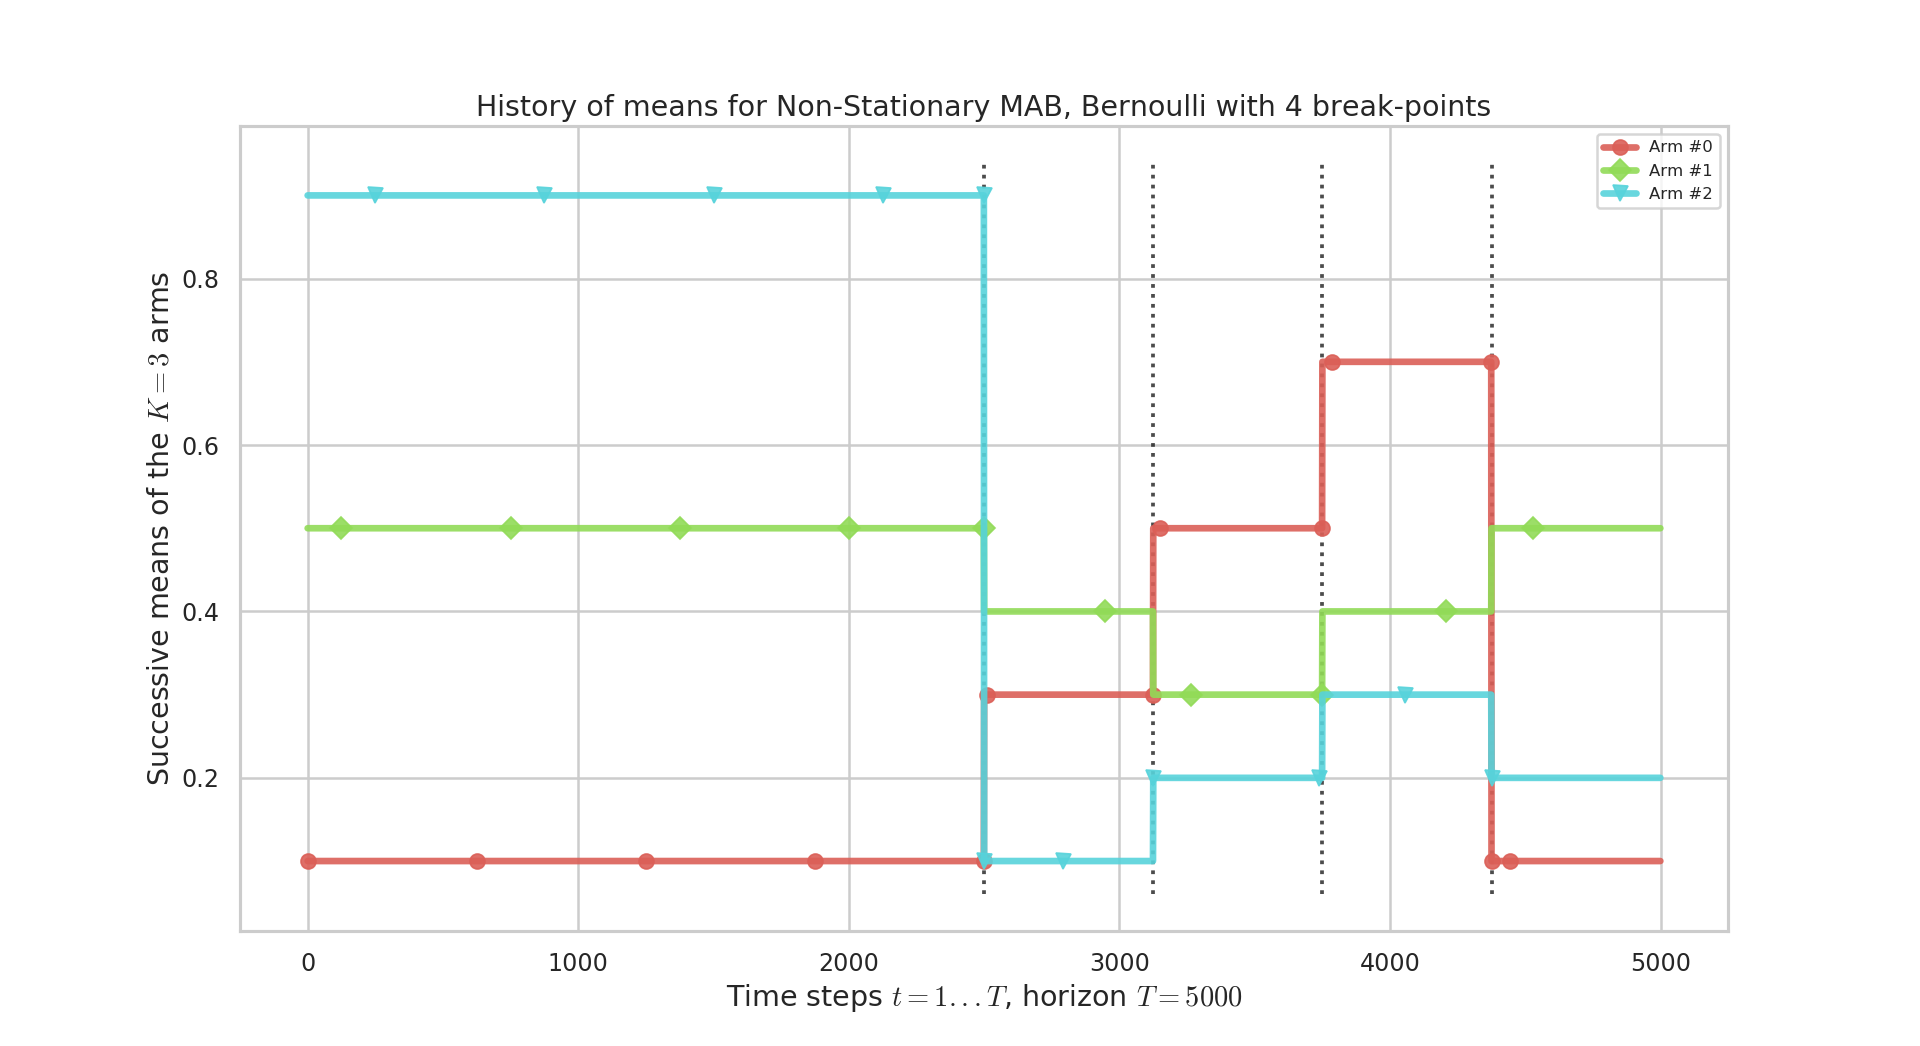
\includegraphics[width=0.80\linewidth]{2-Chapters/6-Chapter/nonstatbandits.git/figures/6_Problems/Problem_4.pdf}
    \caption{\textbf{Problem 4}: $K=3$ arms with $T=5000$, $\Upsilon=4$ changes occur on all arms at a time (\ie, $C=12$).}
    \label{fig:6:Problem_4}
\end{figure}


% - Pb 6 is Yahoo! example from Figure~3 in CUSUM-UCB paper \cite{LiuLeeShroff17}
\paragraph{Problem 5.}

Like problem $3$, this hard problem is inspired from synthetic data obtained from a real-world database of clicks from \emph{Yahoo!} (see Figure~3 from \cite{LiuLeeShroff17}).
It is harder, with $\Upsilon=81$ change-points on $K=5$ arms for a longer horizon of $T=100000$.
Some arms change at almost every time steps, for a total number of breakpoints $C=179$, but the optimal arm is almost always the same one (\textcolor{red}{arm $0$, with $\bullet$}).
It is a good benchmark to see if the actively adaptive policies do not detect \emph{too many changes}, as the Oracle-Restart policy suffers higher regret in comparison to \klUCB.
Means are also bounded in $[0.01, 0.07]$, with small gaps of amplitude ranging from $0.02$ to $0.001$,
as shown in Figure~\ref{fig:6:Problem_6}.

\begin{figure}[h!]  % [htbp]
    \centering
    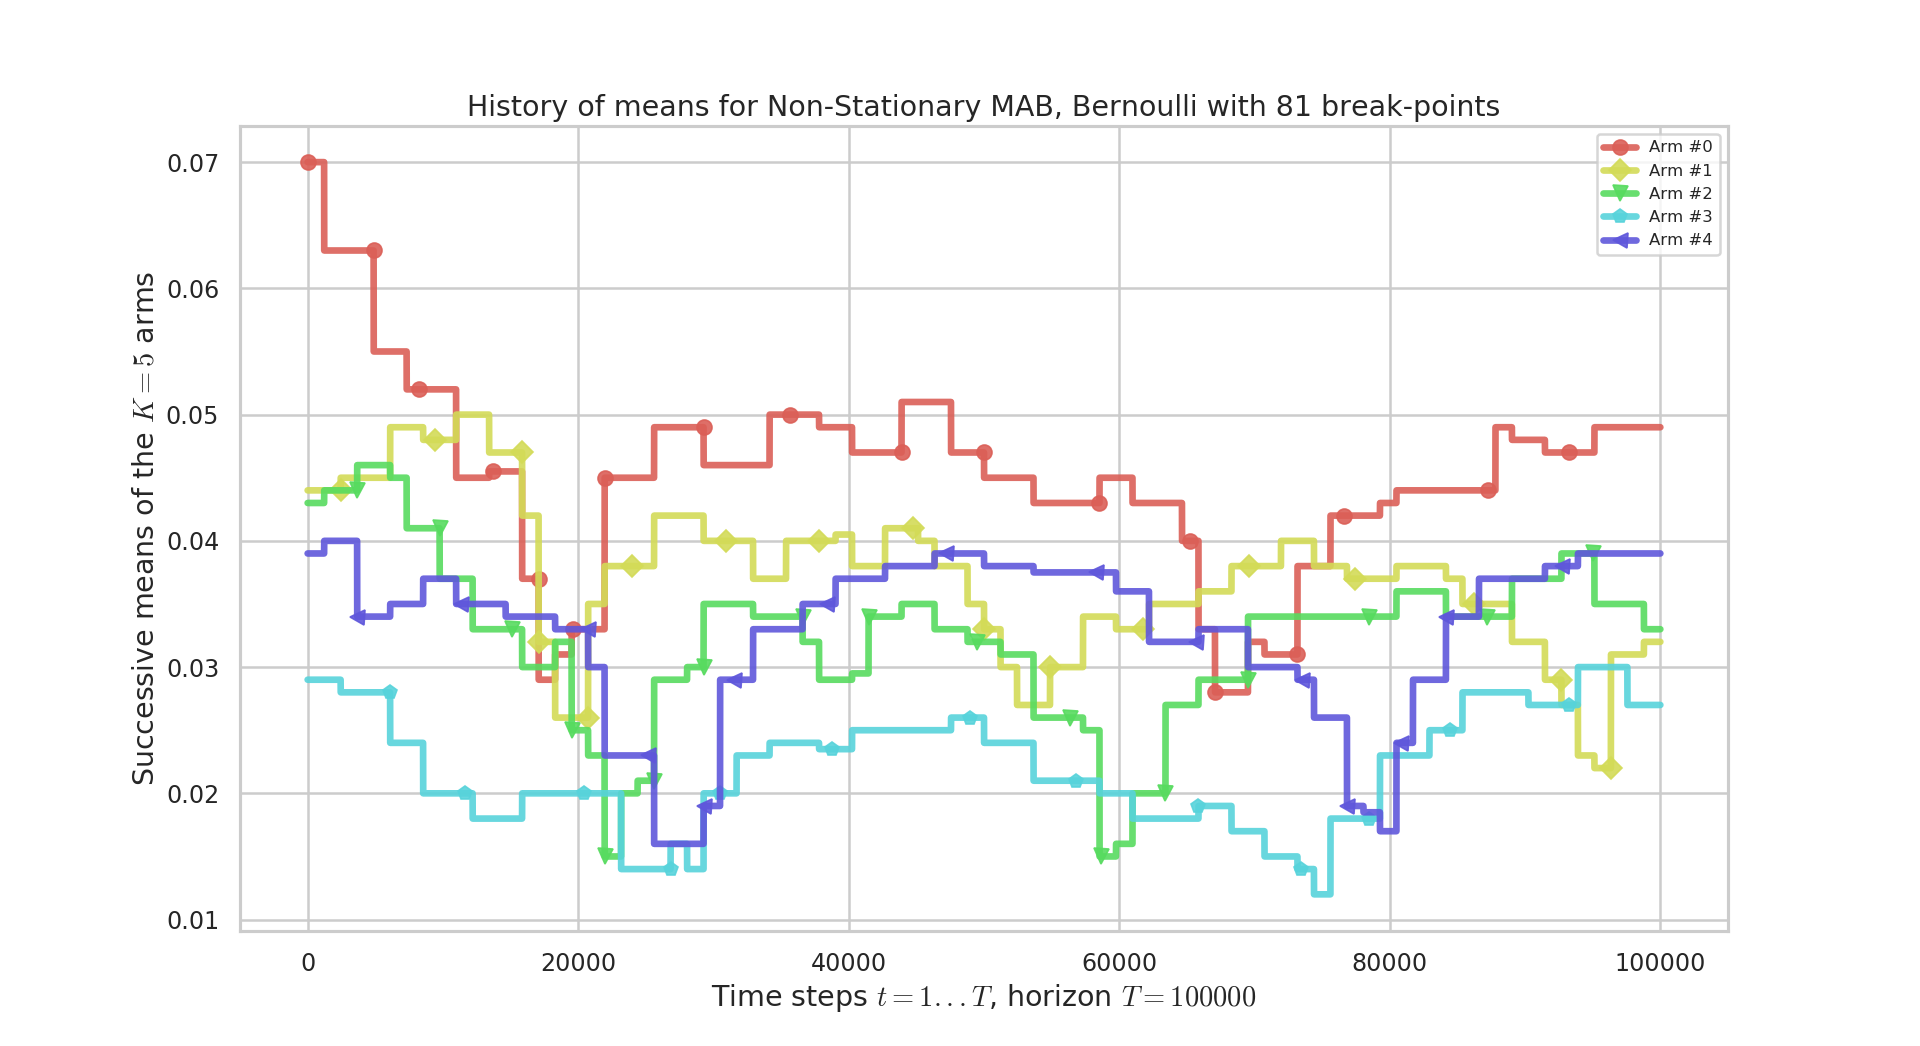
\includegraphics[width=0.80\linewidth]{2-Chapters/6-Chapter/nonstatbandits.git/figures/6_Problems/Problem_6.pdf}
    \caption{\textbf{Problem 5}: $K=5$, $T=100000$, $\Upsilon=81$ changes occurring on some arms at every time ($C=179$).
    }
    \label{fig:6:Problem_6}
\end{figure}


\paragraph{Interpretations.}
%
We include below the figures showing the simulation results for the $5$ problems presented in Section~\ref{sec:6:NumericalExperiments} and Section~\ref{sub:6:TwoMoreProblems}.
The results in terms of mean regret $R_T$ are given in Tables~\ref{table:6:totalResults1} and \ref{table:6:totalResults2}, but it is also interesting to observe two plots for each experiments.
%
First, we show the mean regret as a function of time (\ie, $R_t$ for $1 \leq t \leq T$), for the $9$ algorithms considered (Discounted-\klUCB{} is removed as it is always the most inefficient and suffers high regret).
%
Efficient stationary algorithms, like TS and \klUCB, typically suffer a linear regret after a change on the optimal arm changes if they had ``too'' many samples before the change-points (\eg, on Figure~\ref{fig:6:meanRegretPb1} and even more on Figures~\ref{fig:6:meanRegretPb4} and \ref{fig:6:meanRegretPb5}).
This illustrates the conjecture that classical algorithms can suffer linear regret even on simple piece-wise stationary problems.

On very simple problems, like problem 1, all the algorithms being designed for piece-wise stationary environments perform similarly, but as soon as the gaps are smaller or there is more changes, we clearly observe that our approach \GLRklUCB{} can outperform the two other actively adaptive algorithms \CUSUMklUCB{} and \MklUCB{} (\eg, on Figure~\ref{fig:6:meanRegretPb2}), and performs much more than passively adaptive algorithms DTS and SW-\klUCB{}  (\eg, on Figure~\ref{fig:6:meanRegretPb3}).
Our approach, with the two options of \textbf{Local} or \textbf{Global} restarts, performs very closely to the oracle for problem $4$.

Finally, in the case of hard problems, like problems $3$ and $5$, that have a lot of changes but where the optimal arm barely changes, we verify in Figure~\ref{fig:6:meanRegretPb5} that \klUCB{} and TS can outperform the oracle policy.
Indeed the oracle policy is suboptimal as it restarts as soon as one arm change but is unaware of the meaningful changes, and stationary policies which quickly identify the best arm will play it most of the times, achieving a smaller regret.
We note that, sadly, all actively adaptive policies fail to outperform stationary policies on such hard problems, because they do not observe enough rewards from each arm between two restarts (\ie, the Assumptions~\ref{ass:6:LongPeriodsGlobal} and \ref{ass:6:LongPeriods} for our Theorems~\ref{thm:6:mainRegretBoundGlobal} and \ref{thm:6:mainRegretBound} are not satisfied).
We can also verify that the two options, \textbf{Local} and \textbf{Global} restart, for \GLRklUCB, give close results, and that the \textbf{Local} option is always better.

We also show the empirical distribution of the regret $R_T$, on Figure~\ref{fig:6:histogramRegretPb1}. It shows that all algorithms have a rather small variance on their regret, except Thompson Sampling which has a large tail due to its large mean regret on this (easy) non-stationary problems.


\begin{table}[ht]
    % \begin{small}
    \centering
    \begin{tabular}{c|cccccc}
        \textbf{Algorithms} \textbackslash \textbf{Problems} & Pb $4$ ($T=5000$) & Pb $4$ ($T=10000$) & Pb $5$ \\
        \hline
        Oracle-Restart \klUCB{} & $\mathbf{68 \pm 40}$ & $\mathbf{86 \pm 50}$ & $126 \pm 54$ \\
        \hline
        \klUCB{} & $615 \pm 74$ & $1218 \pm 123$ & $106 \pm 36$ \\
        SW-\klUCB{} & $202 \pm 33$ & $322 \pm 47$ & $228 \pm 27$ \\
        Discounted-\klUCB{} & $911 \pm 210$ & $1741 \pm 200$ & $2085 \pm 910$ \\
        \hline
        Thompson sampling & $756 \pm 65$ & $1476 \pm 137$ & $\mathbf{88 \pm 39}$ \\
        DTS & $250 \pm 39$ & $481 \pm 58$ & $238 \pm 24$ \\
        \hline
        \MklUCB{} & $337 \pm 46$ & $544 \pm 47$ & $116 \pm 36$ \\
        \CUSUMklUCB{} & $267 \pm 69$ & $343 \pm 94$ & $117 \pm 34$ \\
        \hline
        \GLRklUCB{}(Local) & $\mathbf{99 \pm 32}$ & $\mathbf{128 \pm 42}$ & $149 \pm 34$ \\
        \GLRklUCB{}(Global) & $128 \pm 32$ & $185 \pm 47$ & $152 \pm 32$
    \end{tabular}
    \caption{Mean regret $\pm$ $1$ std-dev. Problem $4$ use $K=3$ arms, and a first long stationary sequence. Problem $5$ use $K=5$, $T=20000$ and is much harder with $\Upsilon=82$ breakpoints and $C=179$ changes.}
    \label{table:6:totalResults2}
    % \end{small}
\end{table}


\begin{figure}[h!]  % [htbp]
    \centering
    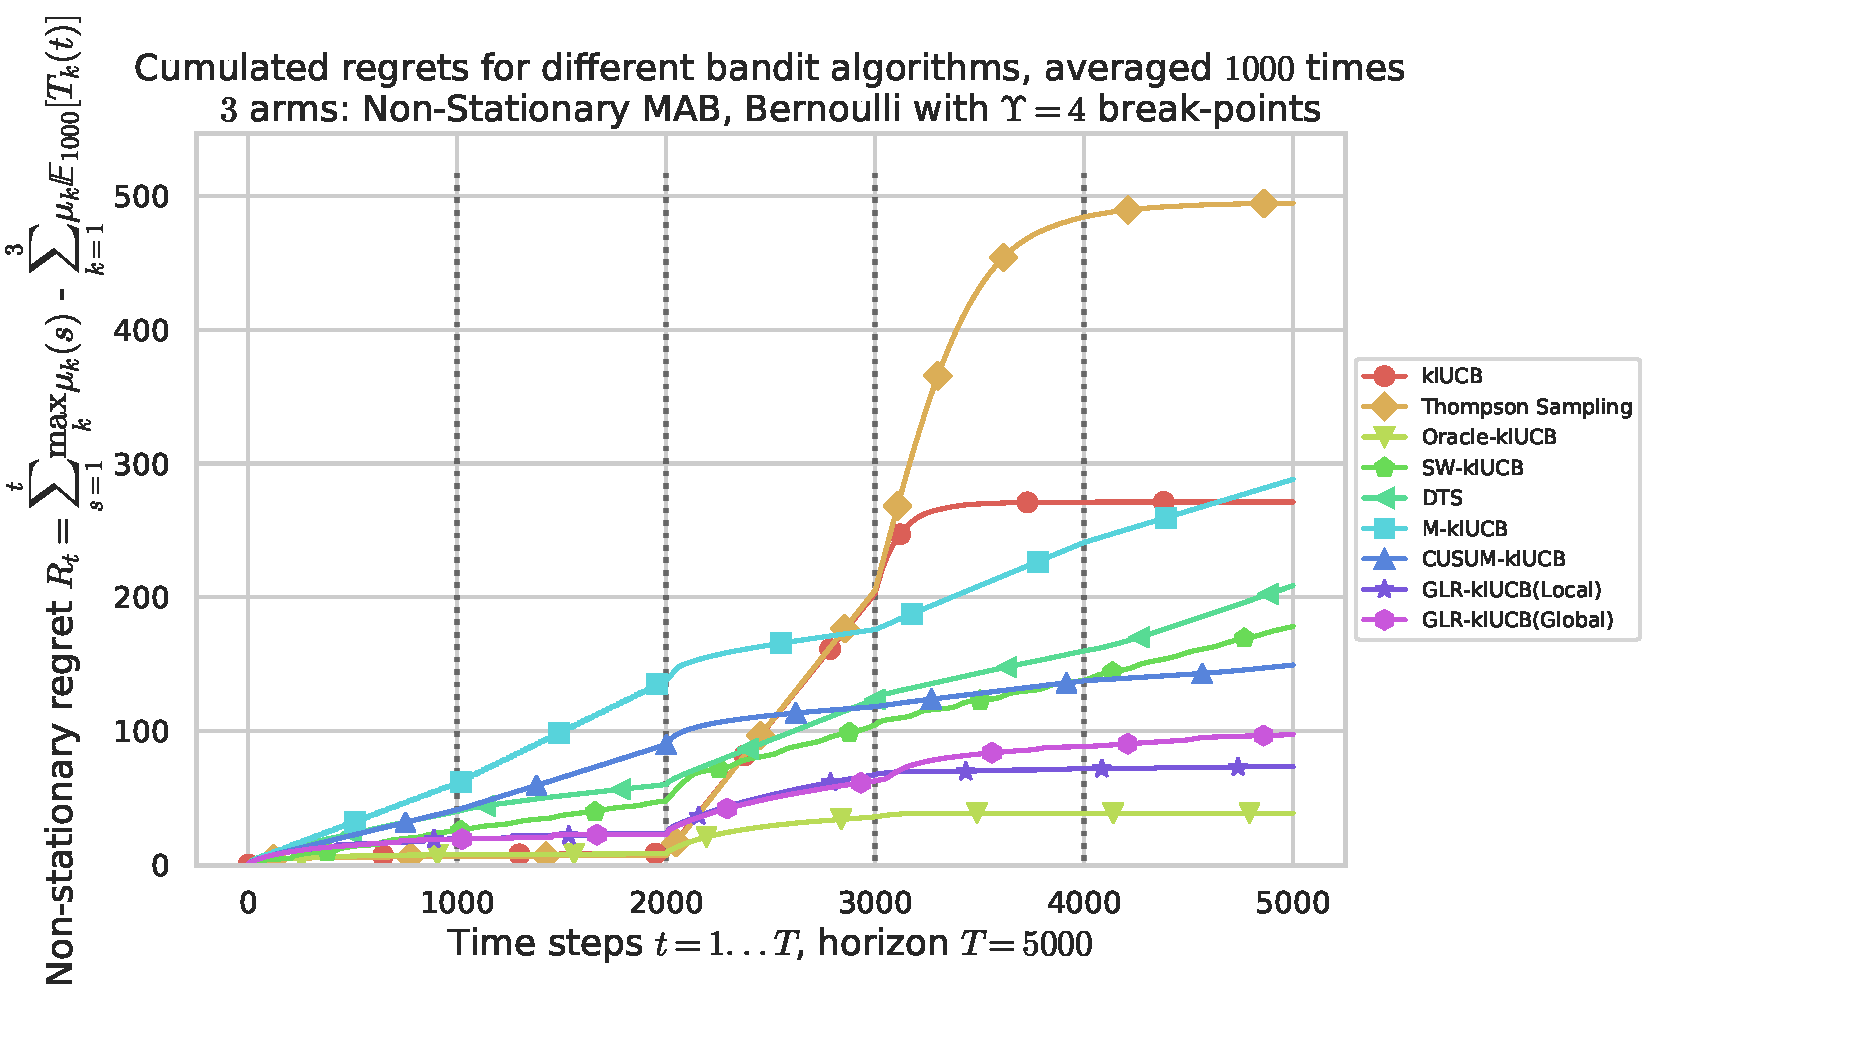
\includegraphics[width=1.00\linewidth]{2-Chapters/6-Chapter/nonstatbandits.git/figures/SP__K3_T5000_N1000__9_algos_pb1/main____env1-1_1316297932259102962.pdf}
    \caption{Mean regret as a function of time, $R_t$ ($1 \leq t \leq T = 5000$) for problem 1.}
    \label{fig:6:meanRegretPb1}
\end{figure}

\begin{figure}[h!]  % [htbp]
    \centering
    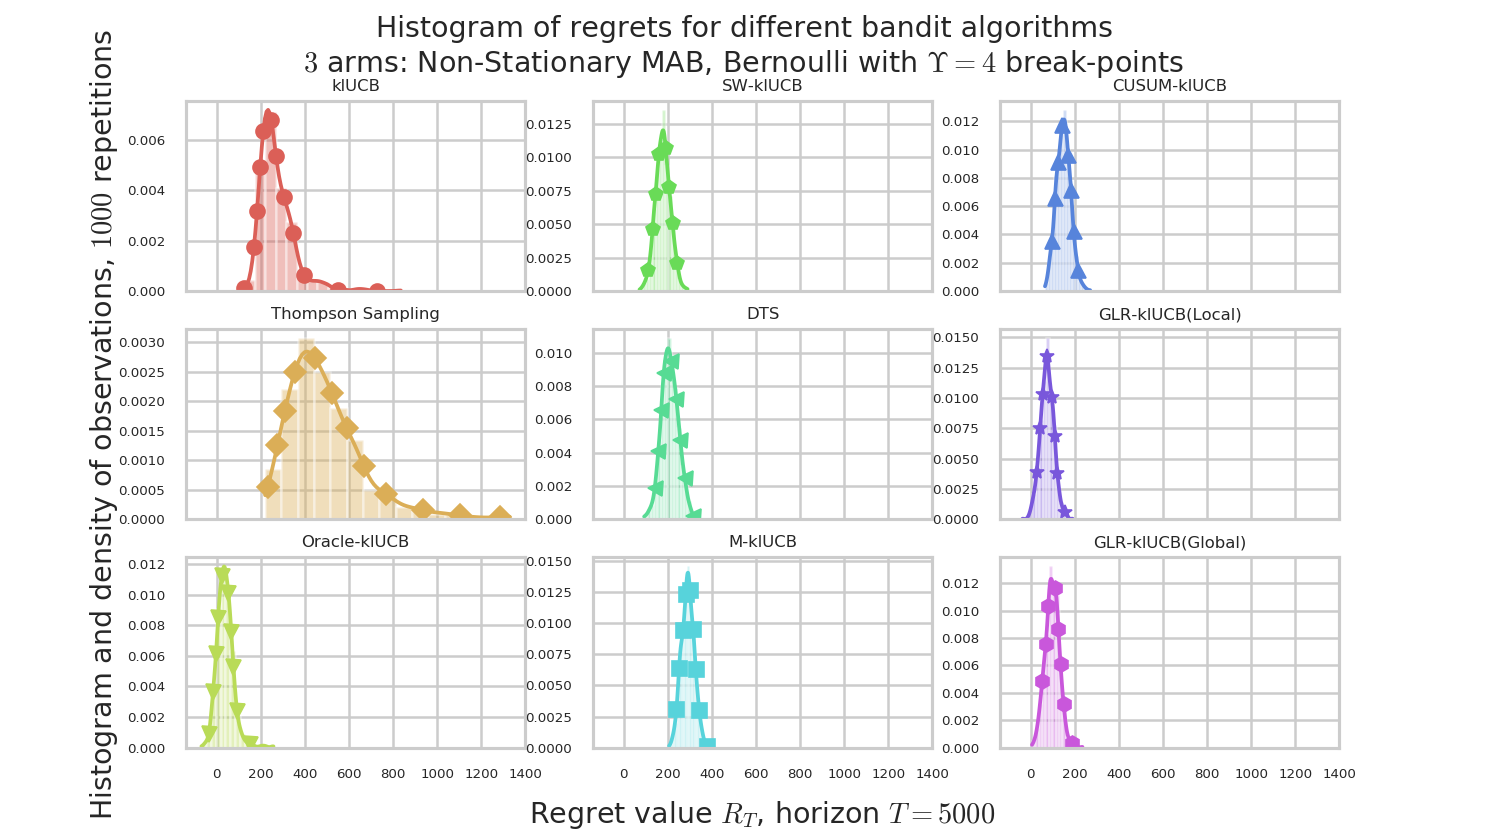
\includegraphics[width=1.00\linewidth]{2-Chapters/6-Chapter/nonstatbandits.git/figures/SP__K3_T5000_N1000__9_algos_pb1/main_HistogramsRegret_shareX____env1-1_1316297932259102962.pdf}
    \caption{Histograms of the distributions of regret $R_T$ ($T=5000$) for problem 1.}
    \label{fig:6:histogramRegretPb1}
\end{figure}

\begin{figure}[h!]  % [htbp]
    \centering
    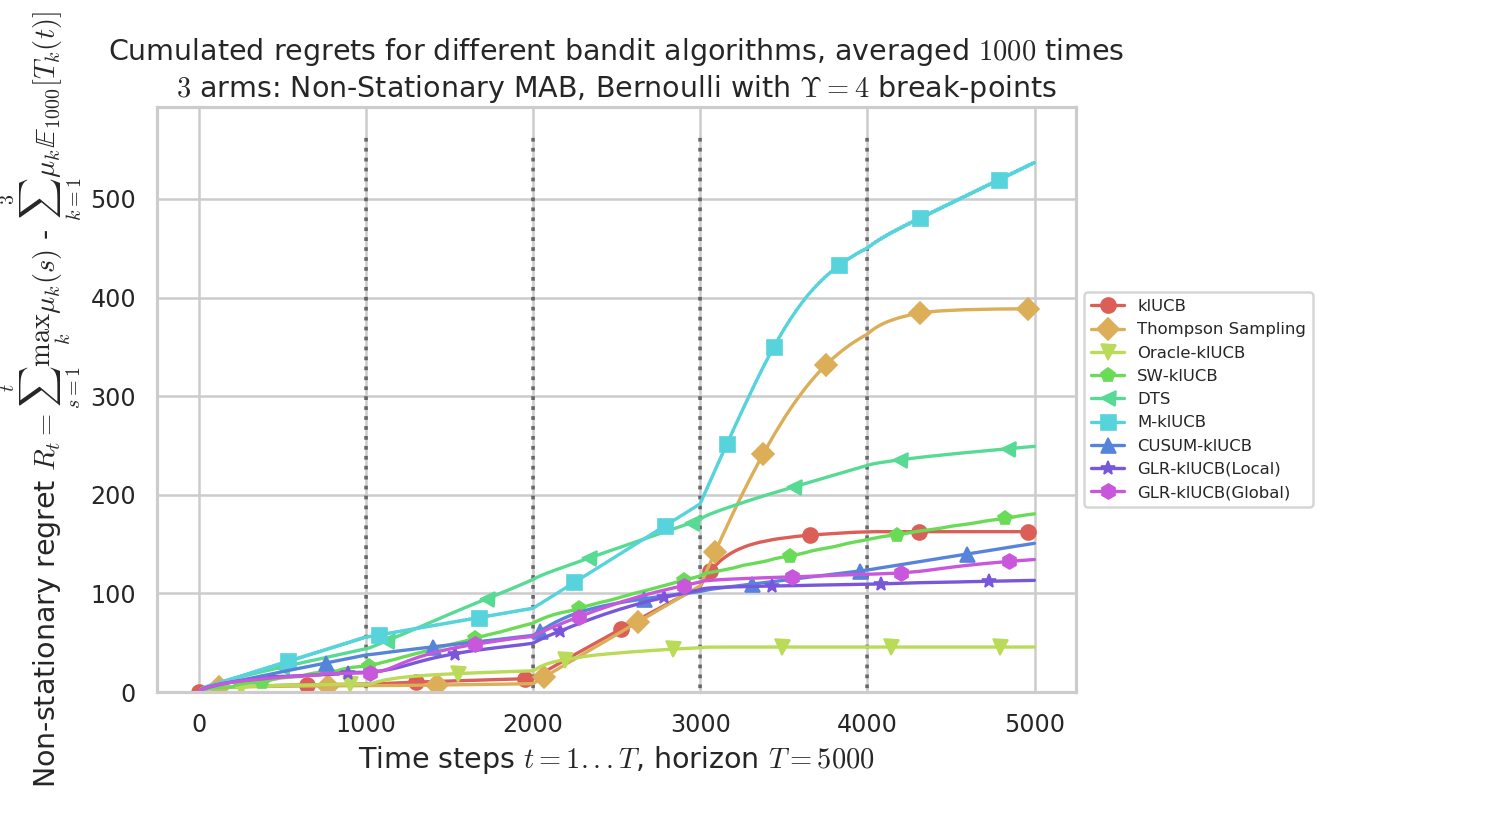
\includegraphics[width=1.00\linewidth]{2-Chapters/6-Chapter/nonstatbandits.git/figures/SP__K3_T5000_N1000__9_algos_pb2/main____env1-1_7882655236216606305.pdf}
    \caption{Mean regret as a function of time, $R_t$ ($1 \leq t \leq T = 5000$) for problem $2$.}
    \label{fig:6:meanRegretPb2}
\end{figure}

\begin{figure}[h!]  % [htbp]
    \centering
    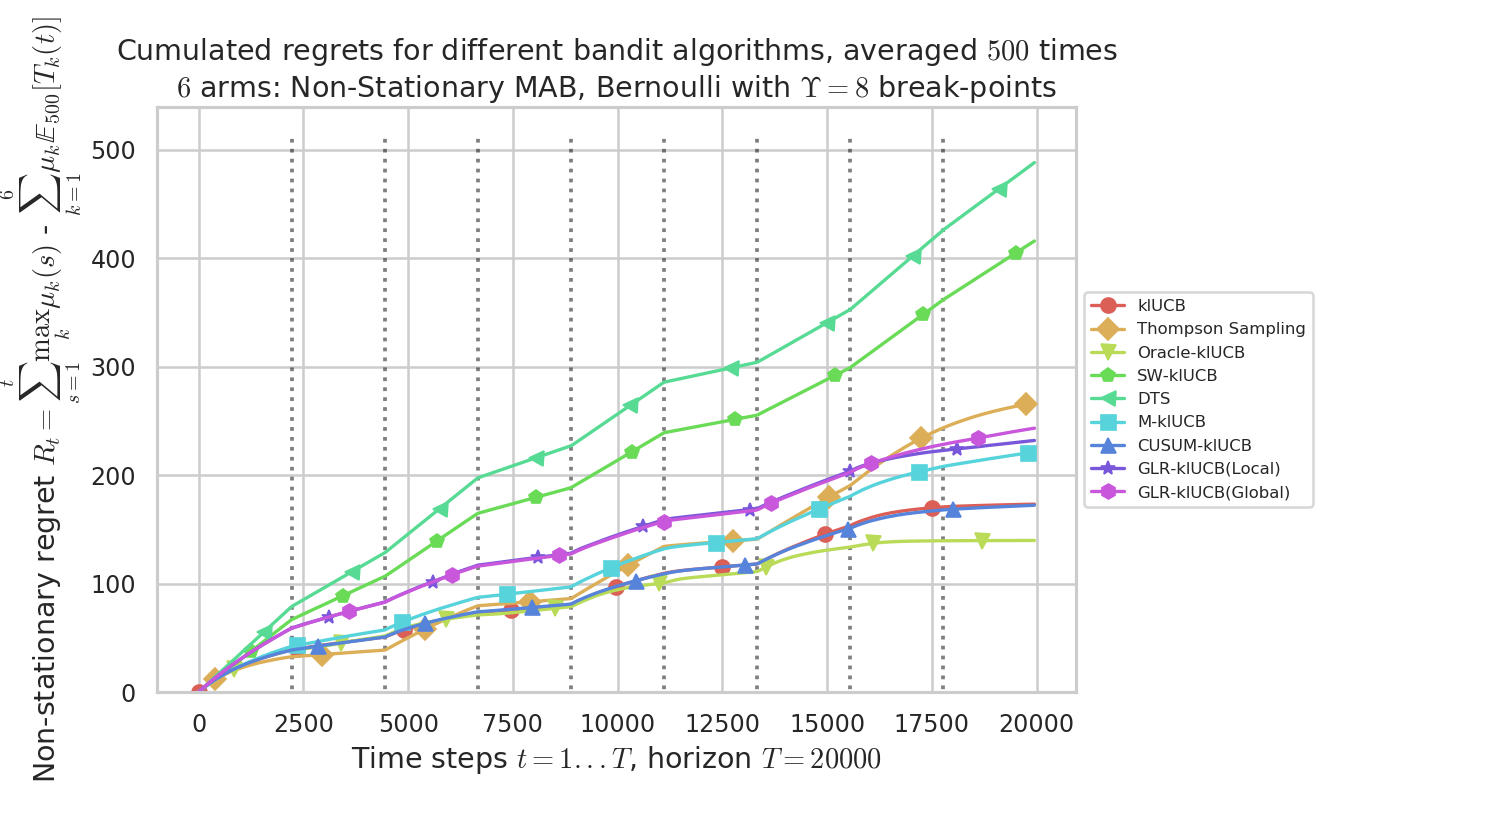
\includegraphics[width=1.00\linewidth]{2-Chapters/6-Chapter/nonstatbandits.git/figures/SP__K6_T20000_N500__9_algos_pb3/main____env1-1_8638317743626238996.pdf}
    \caption{Mean regret as a function of time, $R_t$ ($1 \leq t \leq T = 20000$) for problem 3.}
    \label{fig:6:meanRegretPb3}
\end{figure}

\begin{figure}[h!]  % [htbp]
    \centering
    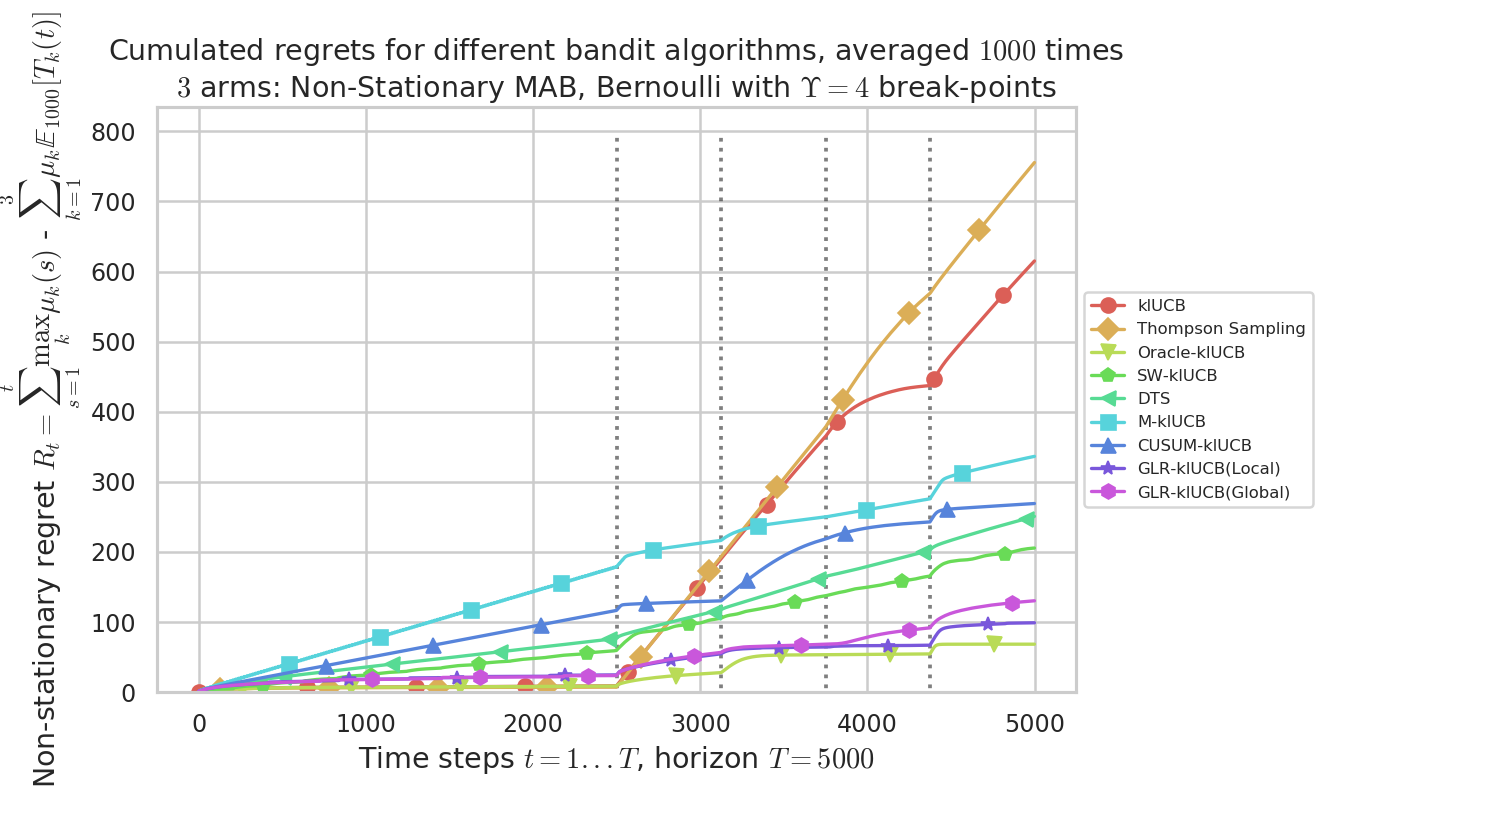
\includegraphics[width=1.00\linewidth]{2-Chapters/6-Chapter/nonstatbandits.git/figures/SP__K3_T5000_N1000__9_algos_pb4/main____env1-1_7471744535647872376.pdf}
    \caption{Mean regret as a function of time, $R_t$ ($1 \leq t \leq T = 5000$) for problem 4.}
    \label{fig:6:meanRegretPb4}
\end{figure}


% -----------------------------------------------------------------
\begin{figure}[h!]  % [htbp]
    \centering
    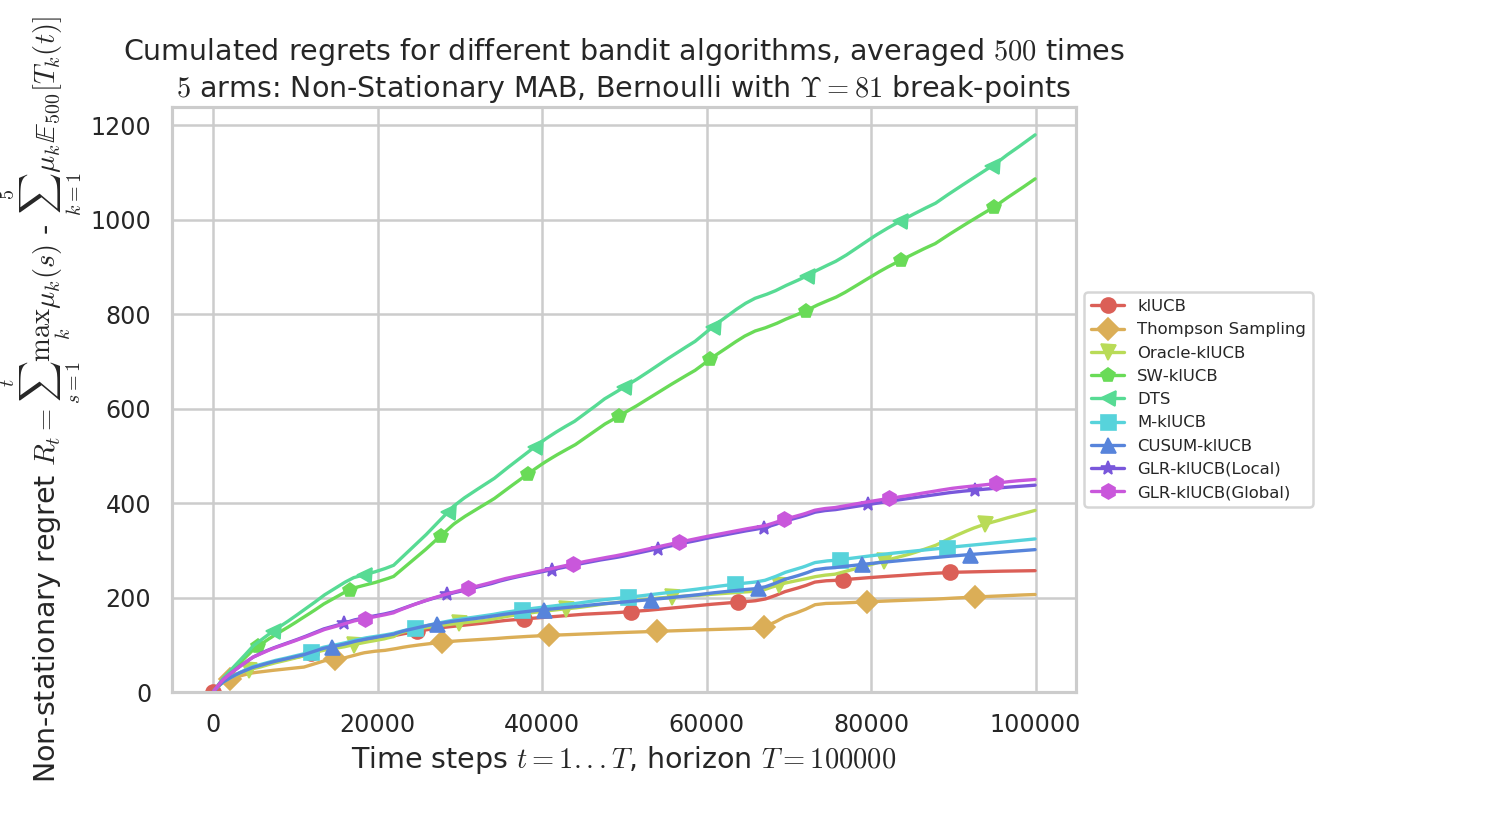
\includegraphics[width=1.00\linewidth]{2-Chapters/6-Chapter/nonstatbandits.git/figures/SP__K5_T100000_N500__9_algos_pb5/main____env1-1_950848333706043320.pdf}
    \caption{Mean regret as a function of time, $R_t$ ($1 \leq t \leq T = 100000$) for problem 5.}
    \label{fig:6:meanRegretPb5}
\end{figure}
